\documentclass[10pt]{article}
\usepackage{multicol}
\usepackage{graphicx}
\usepackage{geometry}
\usepackage{wrapfig}
\usepackage{url}
\usepackage{hyperref}
\usepackage{listings}
\usepackage{color}

\geometry{margin=1in}

\definecolor{light-gray}{gray}{0.95}
\definecolor{codegreen}{rgb}{0,0.6,0}
\definecolor{codegray}{rgb}{0.5,0.5,0.5}
\definecolor{codemauve}{rgb}{0.58,0,0.82}
\lstset {
  language=Python,
  commentstyle=\color{codegreen},
  keywordstyle=\color{blue},
  numberstyle=\color{codegray},
  stringstyle=\color{codemauve},
  basicstyle=\ttfamily,
  columns=fullflexible,
  keepspaces=true
}

\title{Databrowse: An extensible data management platform}
\author{
        Tyler J. Lesthaeghe \\
                Department of Aerospace Engineering and\\
                Center for Nondestructive Evaluation\\
        Iowa State University of Science and Technology\\
        Ames, Iowa 50011\\
        tylerl@iastate.edu
}
\date{\today \\
	Version 0.7}

\newcommand{\confitem}[5]{ 
	\textbf{#1} \texttt{self.#2} (\textit{#3}) \\
	Default: \texttt{#4} \\
	#5\\
	\\
}

\def\changemargin#1#2{\list{}{\rightmargin#2\leftmargin#1}\item[]}
\let\endchangemargin=\endlist 

\begin{document}
\maketitle

\clearpage
\noindent\textbf{Databrowse:  An Exensible Data Management Platform} \\
Copyright \copyright\ 2012-2016 Iowa State University Research Foundation, Inc. \\
All rights reserved.
\hfill\break
\hfill\break
Redistribution and use in source and binary forms, with or without modification, are permitted provided that the following conditions are met:
\begin{enumerate}
\item Redistributions of source code must retain the above copyright notice, this list of conditions and the following disclaimer.
\item Redistributions in binary form must reproduce the above copyright notice, this list of conditions and the following disclaimer in the documentation and/or other materials provided with the distribution.
\item Neither the name of the copyright holder nor the names of its contributors may be used to endorse or promote products derived from this software without specific prior written permission.
\end{enumerate}
THIS SOFTWARE IS PROVIDED BY THE COPYRIGHT HOLDERS AND CONTRIBUTORS ``AS IS'' AND ANY EXPRESS OR IMPLIED WARRANTIES, INCLUDING, BUT NOT LIMITED TO, THE IMPLIED WARRANTIES OF MERCHANTABILITY AND FITNESS FOR A PARTICULAR PURPOSE ARE DISCLAIMED. IN NO EVENT SHALL THE COPYRIGHT HOLDER OR CONTRIBUTORS BE LIABLE FOR ANY DIRECT, INDIRECT, INCIDENTAL, SPECIAL, EXEMPLARY, OR CONSEQUENTIAL DAMAGES (INCLUDING, BUT NOT LIMITED TO, PROCUREMENT OF SUBSTITUTE GOODS OR SERVICES; LOSS OF USE, DATA, OR PROFITS; OR BUSINESS INTERRUPTION) HOWEVER CAUSED AND ON ANY THEORY OF LIABILITY, WHETHER IN CONTRACT, STRICT LIABILITY, OR TORT (INCLUDING NEGLIGENCE OR OTHERWISE) ARISING IN ANY WAY OUT OF THE USE OF THIS SOFTWARE, EVEN IF ADVISED OF THE POSSIBILITY OF SUCH DAMAGE.
\hfill\break
\hfill\break
This material is based on work supported by the Air Force Research Laboratory under Contract \#FA8650-10-D-5210, Task Order \#023, and performed at Iowa State University.
\hfill\break
\hfill\break
DISTRIBUTION A.  Approved for public release:  distribution unlimited; 19 Aug 2016; 88ABW-2016-4051.
\clearpage
\tableofcontents

\clearpage
\section{Introduction}

Databrowse is an extensible web-based platform for data viewing, manipulation, and management.  At the most basic level, Databrowse is a file browser; however, simple plugins enable Databrowse to represent data of a variety of formats in a consistent way, enabling rapid viewing and transformation of those views to narrow in on features of interest.  The plugin architecture enables Databrowse to be adapted to support any data format in which knowledge of the data format is available.  Data from multiple sources or formats can be pulled together into combined representations and then further transformed as desired.  Furthermore, all of these transformations are performed in real time.

\subsection{Motivation}

Databrowse was originally developed to aid in viewing and analyzing data collected in the field of nondestructive evaluation (NDE).  NDE is a broad, highly interdisciplinary field related to the development of measurement techniques that find and characterize material flaws and condition.  Some well known NDE techniques include visual/liquid penetrant inspection, magnetic particle inspection, ultrasonics, radiography, and eddy current testing.  

NDE techniques are capable of generating considerable amounts of data in very short periods of time.  However, many industrial NDE inspections today produce a simple pass/fail response as a result of a testing process.  Recorded raw data is often viewed as useless, or potentially even a liability, unless we have ways to extract useful information.  Ultimately, the problem of finding a needle in a haystack is particularly challenging, especially if you do not know what you are looking for.

Even in research scenarios where we desire to collect large quantities of data to examine specific items, handling large quantities of data can still be a challenge.  As a part of a recent modeling effort related to development of a forward model for vibrothermography, a nondestructive testing technique that utilizes vibration-induced heating to located cracks in materials, the need became apparent for better tools and data management practices.  It was known at the beginning of the work that a considerable amount of data was to be generated.  In the end, a final data table containing almost 25,000 entries was generated, along with over 0.5 TB of raw data.  

The authors sought to develop a tool that would help in the short term for dealing with the latter problem, while serving as a spring board to further work toward dealing with the former problem.  Databrowse was the resulting tool.

\subsection{Implementation}

\subsubsection{XML}

\begin{figure}
	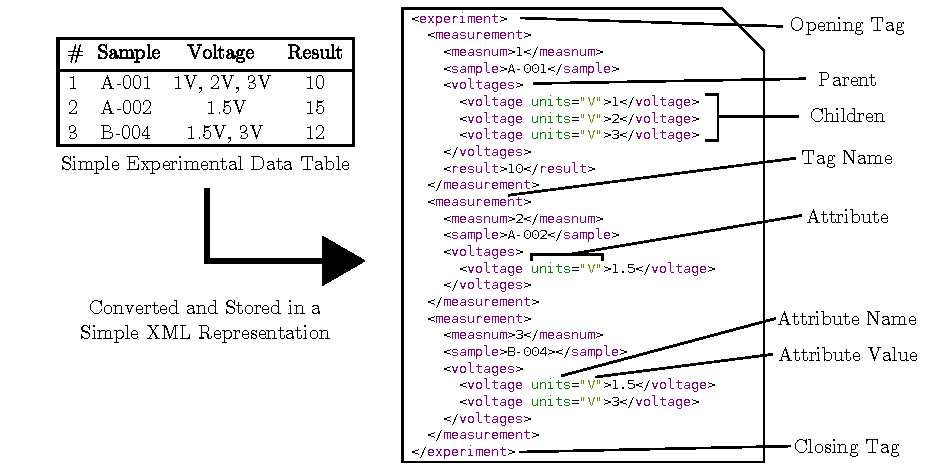
\includegraphics{Chapter4_XMLSample.pdf}
	\caption{Sample XML Data}
	\label{fig:4:xmlsample}
\end{figure}

Databrowse represents data as XML.  XML (eXtensible Markup Language) is a standard that allows text data to be hierarchically structured utilizing arbitrarily defined tags.  Special engines can then be used to parse and manipulate such structured data.  Figure \ref{fig:4:xmlsample} shows an example of a simple data set being structured and stored in an XML format.  The first line of the sample XML file shows an experiment tag, and the last line shows that tag being closed.  Everything contained between the opening and closing tags can be described as children.  In this context, our measurements are children of the experiment.  Thus, a hierarchical data structure can be developed.  Subsequently, we have represented all of the individual parameters for each measurement as children of that measurement.  

We can take it a step further and indicate that one of these parameters could have multiple values, as seen with the voltage data.  This is one major advantage of this type of data structure, as our spreadsheet style data table does not necessarily make representing this type of data structure easy.  We have made it work here with a comma list of values in our data table; however, this does not work so easily with more complicated data.

Furthermore, XML tends to work very nicely as a way of representing most data, since many frequently used data formats internally represent data in a natural hierarchical structure, often as a convenient way of dealing with the issue just described.  Therefore, conversion to XML, if even required, is generally very straightforward.  Once represented as XML, Databrowse is able to leverage the power and speed of the open source XML engine libxml2.  The result is being able to parse and transform considerable amounts of data in seconds.

It is important to note that raw binary waveforms are not intended to be represented as XML; however, pieces of them might be.  More typically though, a plugin would utilize an interface provided by Databrowse that enables the creation of images of such data.  Such an image can be generated in real time and served to the web browser by Databrowse.  This would not be limited to images.  Any format that could be displayed in a web browser could be used, such as videos, animations, or any format that can use a web browser plugin to display.

\subsubsection{XSLT}

\begin{figure}
	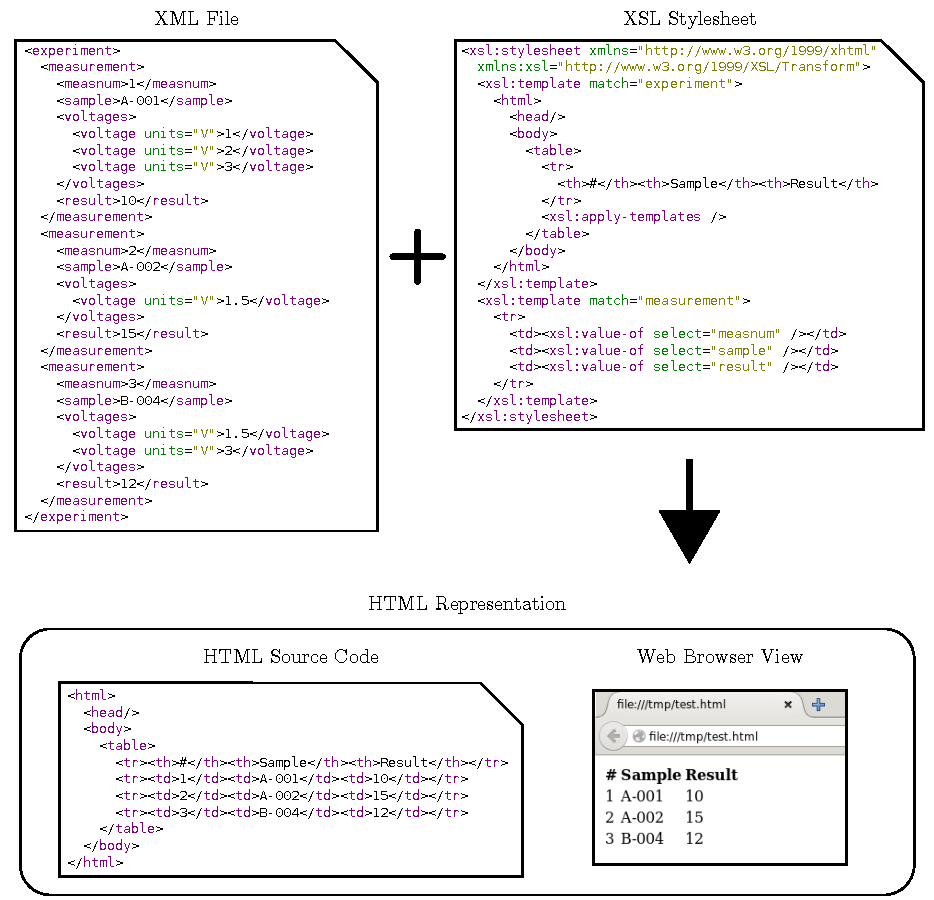
\includegraphics{Chapter4_XSLTSample.pdf}
	\caption{Sample XML Data being Transformed with XSLT}
	\label{fig:4:xsltsample}
\end{figure}

Databrowse utilizes XSLT to transform data.  XSLT (eXtensible Stylesheet Language Template) provides an interface by which the user can define a set of transformations to be applied to XML data.  In other words, XML data and XSLT templates designed to act on that data are provided to the XSLT engine and the engine will output a new set of XML data based on the transformation provided.  This behavior can be seen in Figure \ref{fig:4:xsltsample}, where our sample data from Figure \ref{fig:4:xmlsample} has been transformed using an XSLT template.

Databrowse, being a web based platform, wants to build web pages utilizing the data being provided.  HTML, the language with which web pages are built, is a type of XML.  As a result, our XSLT transform is able to take our data file and build a web page dynamically in real time.  Databrowse then handles the process of serving that web page to a user in their web browser.

\subsection{Databrowse Plugins}

Databrowse plugins are responsible for providing the following:  1) registering the file types with which they should be able to operate on, 2) providing an XML representation of the file, and 3) providing an XSLT transform that converts the XML representation to the desired HTML view that is displayed in the web browser.  Plugins are also able to provide additional features that can be triggered or accessed from the web view.  Such features might include the automatic generation of animations, data conversions, or running of processing scripts.

Since every file can be represented as XML, Databrowse provides an interface for recursively obtaining an XML representation of entire directories and sub-directories.  Thus, a single representation of multiple files can be obtained.  In addition to providing a set of plugins for some common file types, Databrowse includes some plugins designed to provide a simple interface for building such combined representations.  XSLT transformation stylesheets can also be provided on a per-directory basis if additional control is needed for specific use cases.

\clearpage
\section{Installing Databrowse}

\subsection{Software Requirements and Dependencies}

Databrowse requires the use of a WSGI compliant web server.  Databrowse has been tested extensively with mod\_wsgi on Apache 2.2.15 on Red Hat Enterprise Linux 6.6 and Apache 2.4.10 on Ubuntu 15.04.  The usage of mod\_wsgi, Apache, and a Unix-based operating system are strongly recommended.  Using Apache on Windows has been preliminarily tested; however, its use is strongly discouraged at this time due to file path issues that will be resolved in a later version of Databrowse.

Modern versions of Mozilla Firefox and Google Chrome are recommended for accessing Databrowse.  Usage of Microsoft Internet Explorer is strongly discouraged.  Microsoft Edge has not yet been tested.

Databrowse is dependent upon Python 2 (2.6 or later, Python 3 is not supported at this time).  Databrowse also requires the following Python modules (available from PIP or the package management systems on Red Hat and Ubuntu):

\begin{itemize}
	\item python-lxml version 3.2 or greater
	\item python-magic version 0.2 or greater
	\item python-numpy version 1.8 or greater
	\item python-pillow version 2.3 or greater
	
\end{itemize}

Several Databrowse plugins packaged with the distribution also require the use of the following Python modules:

\begin{itemize}
	\item python-qrcode version 4.0 or greater
	\item Dataguzzler Python Bindings (\url{http://thermal.cnde.iastate.edu/dataguzzler})
	\item Dataguzzler Units Support (\url{http://thermal.cnde.iastate.edu/dataguzzler})
\end{itemize}

Databrowse also requires the use of mod\_rewrite for URL rewriting.  Databrowse can be ran without this support enabled; however, its use has not been tested extensively.

\subsubsection{Experimental Windows Use}

A set of binary packages providing the necessary prerequisites have been compiled and are available upon request for usage with Apache on Windows.  These packages require the usage of Apache compiled against the Microsoft Visual C++ 9 Runtime.  This is a limitation imposed by Python 2.  WampServer 2.2d is one such binary distribution of Apache that meets these requirements.  Please contact the author for additional information. 

\subsection{Installation on Unix-based Platforms}

The necessary minimum prerequisites can be installed using the following commands on Debian-based platforms:

\begin{verbatim}
sudo apt-get install python2.7 python-lxml python-magic python-numpy python-pip libjpeg \
   libjpeg-dev libfreetype6 libfreetype6-dev zlib1g-dev apache2 libapache2-mod-wsgi     \
   libapache2-mod-rewrite
sudo pip install pillow
\end{verbatim}

And for Fedora-based platforms:

\begin{verbatim}
sudo yum install python python-lxml python-magic python2-numpy python-pip libjpeg-turbo \
   libjpeg-turbo-devel freetype freetype-devel zlib zlib-devel httpd mod_wsgi           \
sudo pip install pillow
\end{verbatim}

Obtain the Databrowse source from the Databrowse website or from the GitHub repository (coming soon).  From within the root directory, run the following command:

\begin{verbatim}
sudo python setup.py install
\end{verbatim}

This will install the Databrowse library components into the the Python site-packages directory.  Ensure that the necessary Apache modules are running and available by running the following command for Debian platforms:

\begin{verbatim}
sudo a2enmod wsgi
sudo a2enmod rewrite
\end{verbatim}

And for Fedora platforms, both modules should be enabled by default.  Verify the presence of the following lines in the file \texttt{/etc/httpd/conf/httpd.conf} or in any files contained in \texttt{/etc/httpd/conf.d/}:

\begin{verbatim}
LoadModule rewrite_module modules/mod_rewrite.so
LoadModule wsgi_module modules/mod_wsgi.so
\end{verbatim}

From the Databrowse source folder, copy the contents of the databrowse\_wsgi folder to an appropriate location.  For example, to install the server components in \path{/var/www/databrowse}, use the following command from within the Databrowse source folder:

\begin{verbatim}
sudo mkdir /var/www/databrowse
sudo cp -a databrowse_wsgi/* /var/www/databrowse/
sudo chmod -R 755 /var/www/databrowse
\end{verbatim}

Apache must now be configured.  If working on a Debian-based system with a newer version of Apache, create the file \path{/etc/apache2/sites-available/databrowse.conf} with the following example contents and adjust as necessary for your system.  On Fedora-based systems, the file name should be \path{/etc/httpd/conf.d/databrowse.conf} with the contents below adjusted as necessary:

\begin{verbatim}
WSGIScriptAlias /databrowse /var/www/databrowse/databrowse.wsgi
Alias /dbres /var/www/databrowse/resources

<Location "/databrowse">
    # Implementation of proper user controls is strongly encouraged!
    # Regardless, REMOTE_USER header must be set.
    AuthBasicFake demouser

    # Require SSL is also Strongly Encouraged But Must Be Appropriately Configured
    SSLRequireSSL

    Options FollowSymLinks

    # Rewrite Rules - No Modification Should Be Needed Unless You Change Location Above
    RewriteEngine on
    RedirectMatch ^databrowse$ /databrowse/
    RewriteCond %{QUERY_STRING} path=
    RewriteRule ^(.*)/databrowse\.wsgi(.*)$ $1/databrowse.wsgi [QSA]
    RedirectMatch ^databrowse$ /databrowse/
    RewriteCond %{QUERY_STRING} !path=
    RewriteRule ^(.*)/databrowse\.wsgi(.*)$ $1/databrowse.wsgi?path=/$2 [QSA,L]
</Location>
\end{verbatim}

\textbf{WARNING!}  Improper configuration of a web server can leave your computer and data at risk of exposure.  Databrowse does not provide any built-in authentication mechanism nor should it be relied on to prevent access to files outside of the configured data root.  Accordingly, usage of Databrowse on computer systems in which web server access is available from the Internet is strongly discouraged without the usage of SSL and an appropriate Apache authorization module.  It is strongly encouraged that anyone deploying Databrowse for use over the Internet be comfortable with securely configuring and using Apache.  The authors provide no warranty and are not responsible for loss or damages.  Please see the Databrowse license for additional information.

The above configuration assumes that the Databrowse WSGI components are installed in \path{/var/www/databrowse} and will serve Databrowse from \url{http://localhost/databrowse} and will serve Databrowse static resources from \url{http://localhost/dbres} on a default installation of Apache on Debian-based systems.  The above configuration will utilize server default access permissions, so, you may wish to add additional configuration or ensure that your web server is not accessible from the Internet.  Refer to the warning above.

The following command is required for Debian-based systems only and can be used to enable Databrowse:

\begin{verbatim}
sudo a2ensite databrowse.conf
\end{verbatim}

Prior to restarting Apache, the files \texttt{databrowse\_wsgi.conf} and \texttt{databrowse\_style.xml} (or symbolic links to these files) must exist in the same directory as \texttt{databrowse.wsgi}.  It should be sufficient to simply rename the file \texttt{databrowse\_style.sample.xml} to \texttt{databrowse\_style.xml} until you are ready to customize the appearance of Databrowse.  The \texttt{databrowse\_wsgi.conf} file will require some additional configuration.  A sample file \texttt{databrowse\_wsgi.sample.conf} is provided.

The most critical line that must be changed in \texttt{databrowse\_wsgi.conf} from the sample provided file is \texttt{self.dataroot}.  This should be set to the absolute path of the directory containing the data you wish Databrowse to serve.  Databrowse provides very simple checks to keep the user inside directories below this path; however, this should not be used as a method of security!  Symbolic links pointing out of this directory will be followed and there may be other methods available for a user to escape out of the data root path.

It is also worth noting that files contained within data root must be at least readable by the web server process owner.  To take advantage of the full capabilities of Databrowse, you will also want write access available to the web server process owner as well.  Again, use caution when using Databrowse, especially if you are not familiar with securely configuring Apache.  Additionally, if using SELinux or similar systems, you will need to make additional configuration changes to ensure the web server process has read/write access to all files in the data repository.

Within \texttt{databrowse\_wsgi.conf}, you will also want to ensure that \texttt{self.siteurl} and \texttt{self.resurl} are correct if you have changed any Apache settings from the defaults.  You should also ensure that the directory listed in \texttt{self.checklistpath} has been created within the data root directory.  This setting is related to the Checklist plugin, but, Databrowse presently will not run if this directory does not exist.  This will be corrected in future versions of Databrowse.

Please see Chapter \ref{ConfigOptions} for more information on these files.

Restart the web server and Databrowse should now be ready for use:

\begin{verbatim}
sudo service apache2 restart
\end{verbatim}

You should now be able to access Databrowse by visiting \url{http://localhost/databrowse} in your web browser.

\clearpage
\section{Getting Started}\label{GettingStarted}

This section will provide some information on using the directory interface within Databrowse.

\subsection{Features of Interest}
\begin{figure}[h!]
	\centering
	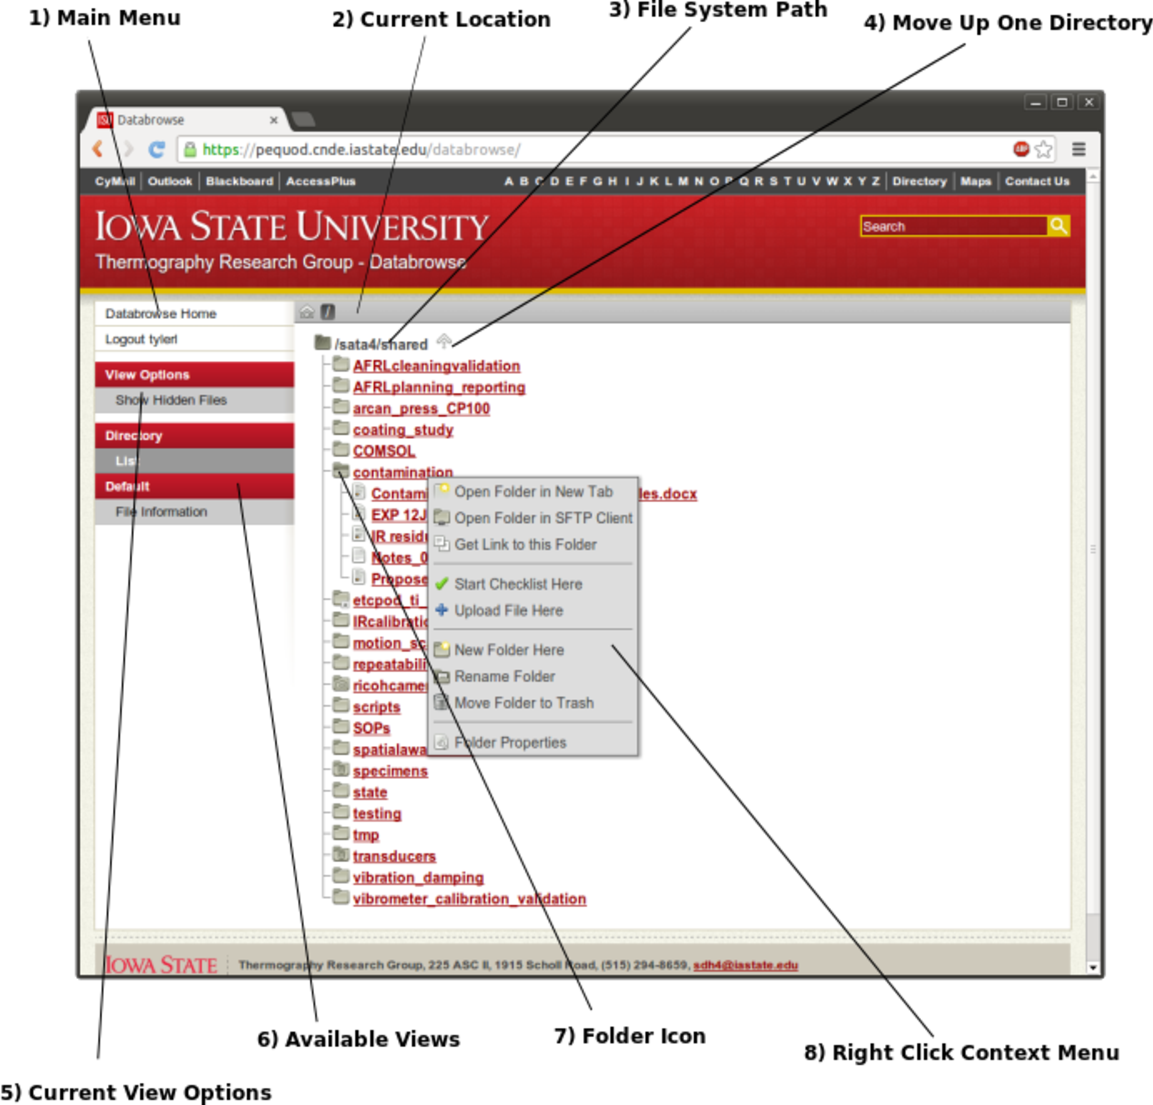
\includegraphics[width=0.8\textwidth]{Overview.pdf}
\end{figure}
\begin{multicols}{2}
\begin{enumerate}
    \item \textbf{Main Menu} \\
          Contains links to jump to the data directory root, logout, and switch views
    \item \textbf{Current Location} \\
          Displays the location of the current view relative to the data directory root -- click a folder name to jump to it
    \item \textbf{File System Path} \\
          Displays the absolute path of the current view in the file system
    \item \textbf{Move Up One Directory} \\
          Click this link to move up one directory until you reach the data directory root
    \item \textbf{Current View Options} \\
          Displays a list of options available to modify the current view
    \item \textbf{Available Views} \\
          Displays a list of various plugins that are capable of rendering the current file or folder and views available within those plugins
    \item \textbf{Folder Icon} \\
          Click this folder icon to expand the folder and dynamically load the contents of the sub folder
    \item \textbf{Right Click Context Menu} \\
          Right click the name of any folder or file in this view to display this context menu
\end{enumerate}
\end{multicols}

\clearpage
\subsection{Creating New Directories}

The following steps can be used to create new directories from Databrowse:

\begin{changemargin}{0in}{150.4pt}
\noindent\textbf{1)} \textbf{Navigate to the Folder that will Contain the New Folder} \newline Using the Databrowse interface, locate the folder that will contain the folder you wish to create.
\end{changemargin}

\begingroup
\setlength\intextsep{0pt}
\begin{wrapfigure}[20]{R}{0.3\textwidth}
		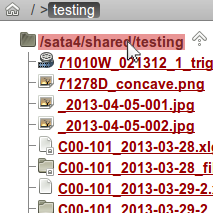
\includegraphics[width=1.9339in]{ContextMenu.png}
\end{wrapfigure}
\noindent\textbf{2)} \textbf{Right Click Folder Name to Open Context Menu} \newline Using the mouse, right click on the name of the folder you wish to contain your new folder.  If the current view is the location you wish to create a new folder within, right click on the black text at the top.  This is the shaded area shown on the figure to the right.

\endgroup

\hfill \break
\hfill \break
\hfill \break
\hfill \break
\hfill \break
\hfill \break
\hfill \break

\begingroup
\setlength\intextsep{0pt}
\begin{wrapfigure}[20]{R}{0.3\textwidth}
		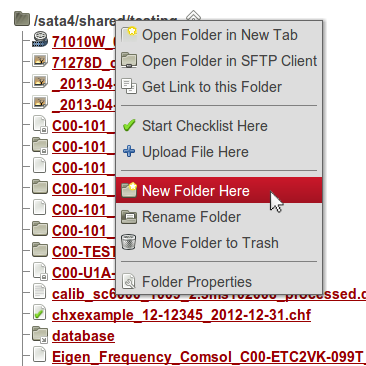
\includegraphics[width=1.9339in]{ContextMenu2.png}
\end{wrapfigure}
\noindent\textbf{3)} \textbf{Select New Folder Here from the Context Menu}

\endgroup

\hfill \break
\hfill \break
\hfill \break
\hfill \break
\hfill \break
\hfill \break
\hfill \break
\hfill \break
\hfill \break
\hfill \break
\hfill \break

\begingroup
\setlength\intextsep{0pt}
\begin{wrapfigure}[20]{R}{0.3\textwidth}
		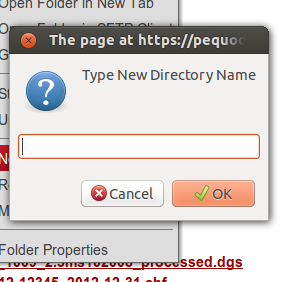
\includegraphics[width=1.9339in]{ContextMenu3.png}
\end{wrapfigure}
\noindent\textbf{4)} \textbf{Type a Name and Click OK} \newline Type a name for your new folder.  Spaces are special characters that are permitted in folder names on your operating system may be used; however, their use is discouraged.

\endgroup

\hfill \break
\hfill \break
\hfill \break
\hfill \break
\hfill \break
\hfill \break
\hfill \break
\hfill \break

\noindent\textbf{5)} \textbf{Finished!} \newline You will be taken to the new folder automatically.

\clearpage
\subsection{Uploading Files}

The following steps can be used to upload files using Databrowse:

\begin{changemargin}{0in}{150.4pt}
\noindent\textbf{1)} \textbf{Navigate to the Folder in which you wish to Upload Files} \newline Using the Databrowse interface, locate the folder that will contain the files you wish to upload.
\end{changemargin}

\begingroup
\setlength\intextsep{0pt}
\begin{wrapfigure}[20]{R}{0.3\textwidth}
		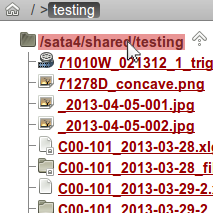
\includegraphics[width=1.9339in]{ContextMenu.png}
\end{wrapfigure}
\noindent\textbf{2)} \textbf{Right Click Folder Name to Open Context Menu} \newline Using the mouse, right click on the name of the folder in which you wish to upload files.  If the current view is the location you wish to upload files to, right click on the black text at the top.  This is the shaded area shown on the figure to the right.

\endgroup

\hfill \break
\hfill \break
\hfill \break
\hfill \break
\hfill \break
\hfill \break

\begin{changemargin}{0in}{150.4pt}
\noindent\textbf{3)} \textbf{Select Upload Files Here from the Context Menu}
\end{changemargin}

\begingroup
\setlength\intextsep{0pt}
\begin{wrapfigure}[20]{R}{0.3\textwidth}
		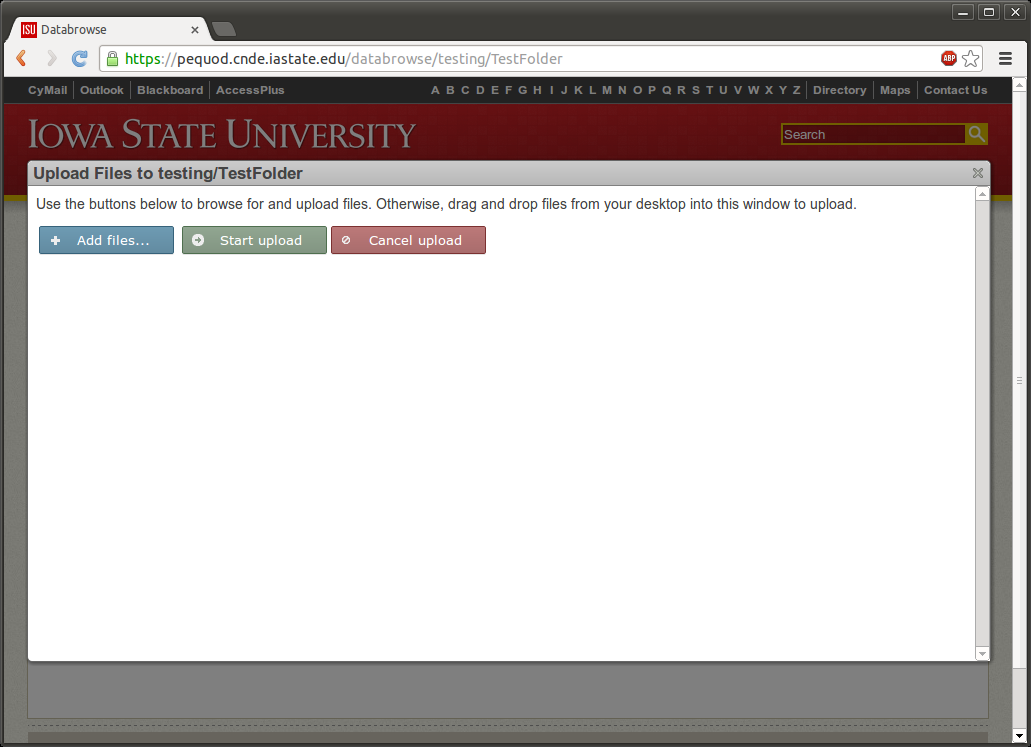
\includegraphics[width=1.9339in]{Upload.png}
\end{wrapfigure}
\noindent\textbf{4)} \textbf{Click Add Files to Open the File Selection Box} \newline Inside the file selection box, you may hold Shift or Ctrl on the keyboard to select multiple files.  Select Open once you have chosen the file(s) you wish to upload.  Repeat for any additional files to be uploaded.  The options you have selected will appear in the window. \newline\newline \textbf{Alternatively, Drag and Drop Files into the Upload Window} \newline Using Windows Explorer, Finder, or Nautilus, depending on your operating system, you may drag files into the open space on the upload window.  The files will appear in the window. 

\endgroup

\hfill \break

\begingroup
\setlength\intextsep{0pt}
\begin{wrapfigure}[20]{R}{0.3\textwidth}
		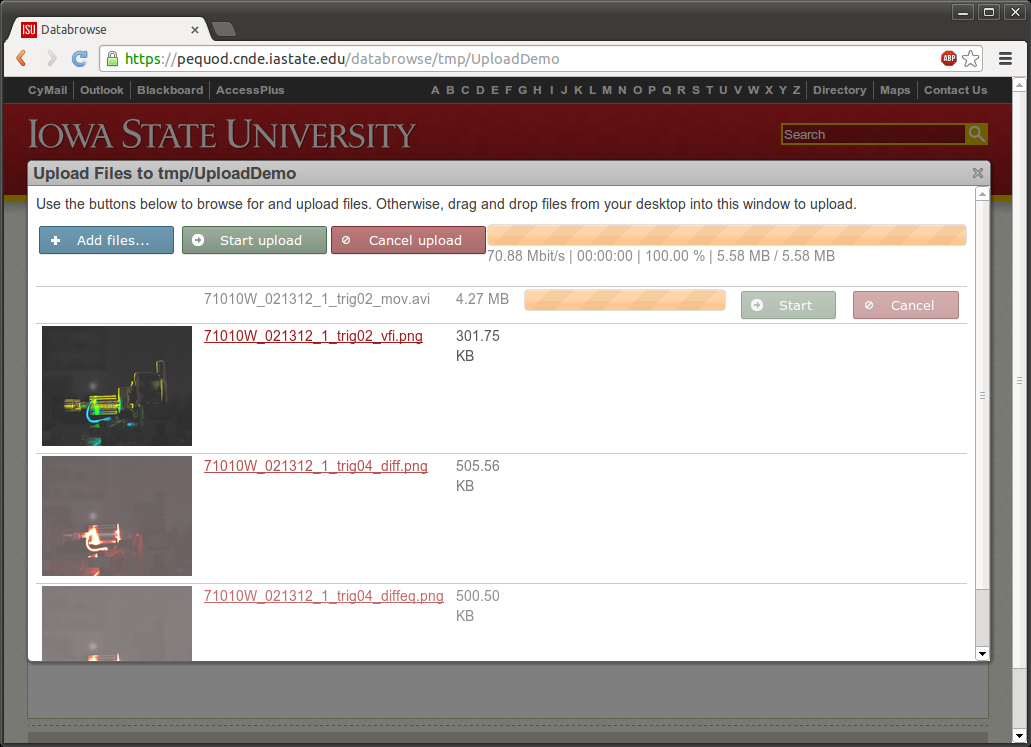
\includegraphics[width=1.9339in]{Upload2.png}
\end{wrapfigure}
\noindent\textbf{5)} \textbf{Click Start Upload} \newline You should see progress bars indicating the length of time remaining to upload your files.  If uploading photos, you will see a preview thumbnail of the photo. 

\endgroup

\hfill \break
\hfill \break
\hfill \break
\hfill \break

\begin{changemargin}{0in}{150.4pt}
\noindent\textbf{6)} \textbf{Click the X or Click Outside of the Upload Window to Close} \newline The page will automatically refresh to show your new files.  Do not close the window while uploading is still taking place or your upload will be interrupted.
\end{changemargin}


\clearpage
\section{Databrowse Configuration Options}
\label{ConfigOptions}

This section provides information about the various configuration options that can be used to customize the low level functionality of Databrowse.

\subsection{\texttt{databrowse\_wsgi.conf}}

The file \texttt{databrowse\_wsgi.conf} (or a symbolic link to this file) must be contained inside the same folder as \path{databrowse.wsgi}.  This file is a Python script that can be used to run code during the start of a web request to the server.  It is ran within the context of the \texttt{web\_support.py} file contained within \texttt{databrowse/support} in the source distribution.  \texttt{web\_support.py} is actually a Python class which is instantiated with the configuration from \texttt{databrowse\_wsgi.conf} and the default values contained within the class at the start of a request.  This code is ran directly during the call to \texttt{web\_support.\_\_init\_\_}.  Accordingly any Python code can be included within \texttt{databrowse\_wsgi.conf} and it will be executed in this context.

The following options can be set in this file:

\smallskip{\vspace{0.25in}}\noindent\confitem{Site URL}{siteurl}{String}{http://localhost/databrowse}{The full URL to Databrowse.  This is used internally to build URLs.  No trailing slash should be used if search engine optimized URLs are enabled.  If you disable search engine optimized URLs, you should update this to list the full URL to \texttt{databrowse.wsgi}.}
\confitem{Resource URL}{resurl}{String}{http://localhost/dbres}{The full URL to Databrowse static resource files.  This is used internally to build URLs to static JavaScript, images, stylesheets, etc.}
\confitem{Logout URL}{logouturl}{String}{http://localhost/logout}{The URL to use in order to trigger the web server's logout mechanism.  This will need to be adjusted depending on your authentication method.}
\confitem{Icon Configuration File}{icondbpath}{String}{\texttt{os.path.join(os.path.dirname(databrowse.support.\_\_file\_\_), "iconmap.conf")}}{The path to a file containing a ConfigParser-compatible configuration file associating file extensions with icons.  See \ref{iconmap} for more information about the contents of this file.}
\confitem{Hidden File Configuration File}{hiddenfiledbpath}{String}{\texttt{os.path.join(os.path.dirname(databrowse.support.\_\_file\_\_), "hiddenfiles.conf")}}{The path to a file containing a ConfigParser-compatible configuration file containing Glob syntax strings that can be used to hide certain files from view in the Databrowse directory views.  See \ref{hiddenfiles} for more information about the contents of this file.}
\confitem{Search Engine Optimization}{seo\_urls}{Boolean}{True}{When set to true, Databrowse will write out URLs that have been search engine optimized.  Instead of the URL \texttt{http://localhost/databrowse.wsgi?path=/SOPs}, the URL would be written as \path{http://localhost/databrowse/SOPs}.  Usage of this feature requires \texttt{mod\_rewrite} to be enabled with the options as suggested in the Installation instructions.  It is strongly encouraged to keep this feature turned on.}
Other options can also be set in this file using the same format, if desired, for use in Databrowse plugins.

\subsection{\texttt{iconmap.conf}}\label{iconmap}

This file generally does not need to be modified, unless you wish to build or modify plugins.  This file tracks the mapping between file types and icons.  These icons are used to provide a graphical representation of a file type within Databrowse.  The file uses a Python ConfigParser module compatible format.  There are two sections that can be used inside this file:  \texttt{[Content-Type]} and \texttt{[Extension]}.  Content types are defined as specified in RFC 2045 and are determined utilizing libmagic.  File extensions are matched against the potion of the filename after the final period.  The content-type or extension becomes the parameter name in \texttt{iconmap.conf} and the parameter value is the name of the file containing the icon served at the URL \texttt{icons/} relative to the Databrowse resources URL (e.g. \texttt{http://localhost/dbres/icons/folder.png}).

The following is an example of how this file is laid out:

\begin{verbatim}
[Content-Type]
inode/directory=folder.png
application/x-directory=folder.png

[Extension]
txt=text-x-generic.png
html=text-html.png
\end{verbatim}

All files that are unable to be matched with a configuration option are given the icon \texttt{unknown.png}.

\subsection{\texttt{hiddenfiles.conf}}\label{hiddenfiles}

This file can be used to hide files based on their file name.  Glob expressions are permitted.  This file uses a Python ConfigParser module compatible format.  There are two sections that can be used inside this file:  \texttt{[Hidden]} and \texttt{[Shown]}.  The hidden section is used to define file names or glob expressions for filenames that should be hidden from the Databrowse directory view.  The shown section can be used to override glob expressions contained in the hidden section for explicit file names.  Glob expressions are also permitted here.  The parameter name is used only for comment and will be ignored by Databrowse.  The parameter value will be used by Databrowse to filter file lists in the directory view.

The following is an example of how this file is laid out:

\begin{verbatim}
[Hidden]
backup_files=*~
hidden_files=.*
generic_backup_files=*.bak

[Shown]
my_special_backup_file=MyBackup*.bak
\end{verbatim}

\clearpage
\section{Databrowse Library}

The core components of Databrowse that are most directly responsible for building XML representations of files and directories are packaged into Python modules.  An interface has been provided that enables Python scripts to leverage the power of Databrowse to quickly obtain XML representations for any file.  This is particularly useful in the context of processing scripts written in Python.  This is also especially useful in contexts in which the Databrowse plugin responsible for handling a particular type of file provides additional information or meta data that wouldn't otherwise be easily accessible working with the file directly.

The Databrowse library can be imported in Python with the following code:

\begin{verbatim}
from databrowse.lib import db_lib as dbl
\end{verbatim}

The library contains one function named \texttt{GetXML}.  This function will return the XML representation of a file, as produced by Databrowse.
\hfill\break
\hfill\break
\noindent \texttt{function dbl.}\textbf{GetXML}\texttt{(filename, output=dbl.OUTPUT\_ELEMENT, **params})
\hfill\break
\hfill\break
\noindent \textbf{Aguments} 
\begin{changemargin}{0.25in}{0in}
\begin{description}
	\item[filename] String containing a relative or absolute path to the file of interest
	\item[output] Determines the type of output to be returned from the function \\
				  \texttt{dbl.OUTPUT\_ELEMENT} returns an LXML etree.Element \\
				  \texttt{dbl.OUTPUT\_ETREE} returns an LXML etree.ElementTree \\
				  \texttt{dbl.OUTPUT\_STRING} returns a string containing the XML \\
				  \texttt{dbl.OUTPUT\_STDOUT} prints the XML string to stdout and returns nothing
    \item[**params] A variable number of optional parameters that are treated the same way as query string values that would be POST or GET to the web server when Databrowse is being used from the web.  Used to pass in various options into plugins.
\end{description}
\end{changemargin}

\noindent \textbf{Usage}
\begin{changemargin}{0.25in}{0in}
\begin{verbatim}
>>> from databrowse.lib import db_lib as dbl
>>> dbl.GetXML('/tmp/emptyfile', output=dbl.OUTPUT_STDOUT)
<default:default>
  <filename>emptyfile</filename>
  <path>/tmp</path>
  <size>0.0 byte</size>
  <mtime>Tue Sep  3 10:12:40 2013</mtime>
  <ctime>Tue Sep  3 10:12:40 2013</ctime>
  <atime>Tue Sep  3 10:12:42 2013</atime>
  <contenttype>text/plain</contenttype>
  <permissions>-rw-rw-r--</permissions>
  <owner>user:user</owner>
</default:default>
\end{verbatim}
\end{changemargin}

It is also worth mentioning the presence of the function \texttt{DebugGetXML} which operates identically to \texttt{GetXML}, however, it launches a Python debugger session, enabling the user to step through the code line by line.

\clearpage
\section{Databrowse Plugin Format}
This section provides documentation on nature of Databrowse plugins.  It is intended to provide enough information that skilled users may be able to build or customize their own Databrowse plugins, but it is not intended to be a tutorial.  Such material will be produced for Databrowse v1.0.

\subsection{Plugin File Structure}
Individual plugins are Python packages contained within the \texttt{databrowse.plugins} namespace.  All plugin names should start with the prefix \texttt{db\_} (this is a legacy requirement and will be removed in Databrowse v1.0).  The file structure of the package should be as follows:

\begin{verbatim}
db_plugin_name\
      __init.py__
      db_plugin_name.py
      dbs_stylesheet_one.xml
      dbs_stylesheet_two.xml
      handlers.py
\end{verbatim}

\subsection{File Contents}
This section will detail the required contents for each file in the plugin.  For the purposes of providing an example, let's say we wish to construct a plugin that simply displays the name of a file to the web page.  This section will display the necessary file contents needed to produce such a plugin.

\subsubsection{\texttt{\_\_init.py\_\_}}
This file does not require any contents.  Its presence is a trigger to the Python interpreter to search for modules.  However, you may find it useful to place a docstring inside this file for usage from the Python console and for documentation purposes.  The presence of a copyright statement is strongly encouraged.  This file can also be used to initialize variables, though, this usage is strongly discouraged in the context of the WSGI server.

\subsubsection{\texttt{db\_plugin\_name.py}}
This file must be named with the same name as the folder name.  The top of the file should contain a copyright statement.  The usage of a docstring at the top of the file is also recommended for identification purposes.  

This file must contain a class derived from \texttt{databrowse.support.renderer\_support.renderer\_class} and named identically to the file name.  It must have several class variables defined:

\begin{description}
	\item[\texttt{\_namespace\_uri}] A string containing the fully qualified URL referring to the XML namespace for the plugin.  Existing Databrowse plugins follow the format \path{http://thermal.cnde.iastate.edu/databrowse/plugin_name}.
	\item[\texttt{\_namespace\_local}] A string containing the local abbreviated form of the namespace.  You should take care to avoid conflicts with other namespace prefixes.
\end{description}

Several other class variables are automatically initialized to defaults, but may be overridden by declaring them as class variables to your inherited class:

\begin{description}
	\item[\texttt{\_default\_content\_mode}] A string identifying the default content mode to be loaded when no content mode is specified.  The content mode \texttt{full} is frequently used.  This serves more as an internal identifier for use within the plugin; however, the content mode \texttt{raw} has special meaning.  This content mode will prevent the main WSGI script from outputting any content to the user.  As a result, you can use the \texttt{raw} content mode to serve binary content to the web browser.  You must manually set the output headers and return content as appropriate from your plugin per PEP 3333.
	\item[\texttt{\_default\_style\_mode}] A string identifying the name of the stylesheet that should be applied to the content output by default if one is not specified by the end user.  This string should not include the \texttt{dbs\_} prefix.  See Section \ref{Stylesheet} for more information.
	\item[\texttt{\_default\_recursion\_depth}] A number indicating how deep a plugin operating on a directory should recurse down a directory tree by default.  This value is not used by plugins that do not operate on directories but should still be set.
\end{description}

An additional set of class variables will be initialized to contain references to objects used by other portions of Databrowse that may be of convenience or use here:

\begin{description}
	\item[\texttt{\_relpath}] A string initialized to the file path of the currently requested file relative to the data root with a leading forward slash.  These paths are used by Databrowse internally to represent full file paths inside URLs.
	\item[\texttt{\_fullpath}] A string initialized to the absolute file path of the currently request file.  This path should be used to access the file.
	\item[\texttt{\_web\_support}] A reference to the instantiated \texttt{web\_support} class, which contains information about the web server request and the current configuration of Databrowse.
	\item[\texttt{\_handler\_support}] A reference to an instantiated \texttt{handler\_support} class, which provides functionality for determining which types of plugins are capable of operating on a particular file.  It also provides support functionality to determine the icon used to represent a file.
	\item[\texttt{\_caller}] A string that identifies the plugin responsible for the call to this plugin.  When set to \texttt{databrowse}, the call to the plugin is the result of a direct request from the Databrowse WSGI application.  Otherwise, this string will contain the name of the plugin making the recursive call to get content from the plugin.  This is most frequently the Directory plugin, which can query a plugin for information about a file.  This information can then be displayed by the Directory plugin as a preview of a file's contents.
	\item[\texttt{\_handlers}] A list of other plugins that are capable of working with this particular type of file, in order of precedence.
\end{description}

The class must contain at least one function -- \texttt{getContent}.  With the exception of the scenario in which the content mode is set to \texttt{raw}, this function must return via with an LXML etree.Element, \texttt{None}, or raise an exception.  The keyword \texttt{None} should only be returned when the plugin is not called by Databrowse, but rather is being called by another plugin.  This is normally the desired behavior, unless your plugin needs to return content to a directory plugin.  The example contents of \texttt{db\_plugin\_name.py} displayed on the following page will produce an XML document containing the filename of the requested file.  The format of the generated XML document is
\begin{lstlisting}[language=XML]
<pn:pn xmlns:pn="http://thermal.cnde.iastate.edu/databrowse/plugin_name">
	<filename>some_file_name.txt</filename>
</pn:pn>
\end{lstlisting}
if the plugin were called with the filename \path{some_file_name.txt}.  This example plugin is trivial, but provides the framework needed to produce XML representations of any type of file.

\clearpage
\begin{lstlisting}
#!/usr/bin/env python
###############################################################################
## Databrowse:  An Extensible Data Management Platform                       ##
## Copyright (C) 2012-2015 Iowa State University                             ##
##                                                                           ##
## This program is free software: you can redistribute it and/or modify      ##
## it under the terms of the GNU General Public License as published by      ##
## the Free Software Foundation, either version 3 of the License, or         ##
## (at your option) any later version.                                       ##
##                                                                           ##
## This program is distributed in the hope that it will be useful,           ##
## but WITHOUT ANY WARRANTY; without even the implied warranty of            ##
## MERCHANTABILITY or FITNESS FOR A PARTICULAR PURPOSE.  See the             ##
## GNU General Public License for more details.                              ##
##                                                                           ##
## You should have received a copy of the GNU General Public License         ##
## along with this program.  If not, see <http://www.gnu.org/licenses/>.     ##
###############################################################################
""" plugins/db_plugin_name/db_plugin_name.py - The Plugin Name Plugin """

from lxml import etree
from databrowse.support.renderer_support import renderer_class


class db_plugin_name(renderer_class):
    """ The Plugin Name Plugin - This plugin is an example """

    _namespace_uri = "http://thermal.cnde.iastate.edu/databrowse/plugin_name"
    _namespace_local = "pn"
    _default_content_mode = "full"
    _default_style_mode = "default_view"
    _default_recursion_depth = 2

    def getContent(self):
        if self._caller != "databrowse":
            return None
        else:
            if self._content_mode == "full":
                xmlroot = etree.Element('{%s}%s' % (self._namespace_uri, self._namespace_local),
                                        nsmap=self.nsmap)
                xmlchild = etree.SubElement(xmlroot, "filename", nsmap=self.nsmap)
                xmlchild.text = os.path.basename(self._fullpath)
                return xmlroot
            else:
                raise self.RendererException("Invalid Content Mode")
        pass
    pass

\end{lstlisting}

\clearpage
\subsubsection{\texttt{dbs\_stylesheet\_name.xml}} \label{Stylesheet}
Plugins can contain any number of XSLT stylesheets that are used to transform the XML content produced by the plugin for a particular file into HTML for display on the web browser.  These stylesheet files must be named with the prefix \texttt{dbs\_} and end with the extension \texttt{.xml}.  Databrowse will automatically locate all stylesheets located within the plugin named in this format and display them as options to the user in the Databrowse menu.  Databrowse will also search for stylesheets inside the data folders placed inside of the \path{.databrowse/stylesheets/db_plugin_name} folder, enabling the end user to write stylesheets for custom views relevant to a particular set of data.  

This file does not contain a complete XSLT stylesheet.  Rather, it contains XSLT template snippets which will be combined with other snippets from other plugins that may be producing content displayed on the page at any given time.  This is particularly important in the context of a directory plugin that is displaying representations of many different files contained within that directory.

This file also does not produce a complete web page.  Rather, it should be written such that it writes out HTML snippets, which will be placed in the appropriate location on the web page.

The construction of an XSLT template and the usage of HTML is outside of the scope of this document.  Please refer to one of many tutorials on the topics available on line.

The following is an example of an XSLT stylesheet that could be used to transform the content produced by the discussed plugin into HTML.

\begin{lstlisting}[language=XSLT]
<xsl:template xmlns="http://www.w3.org/1999/xhtml" 
      xmlns:pn="http://thermal.cnde.iastate.edu/databrowse/plugin_name" 
      xmlns:xsl="http://www.w3.org/1999/XSL/Transform" match="pn:pn" mode="full">
    <h1><xsl:value-of select="filename" /></h1>
</xsl:template>
\end{lstlisting}

\clearpage
\subsubsection{\texttt{handlers.py}}
Plugins must contain a \texttt{handlers.py} file.  This file should contain one function with a name starting with the prefix \texttt{dbh\_}.  The name of this function will be used to determine the order of precedence in ascending order in the case in which multiple plugins can operate on a file.  This function receives three parameters:

\begin{description}
	\item[\texttt{path}] A string containing the full path to the file that has been requested.
	\item[\texttt{contenttype}] A string containing the RFC 2045 compliant MIME type.
	\item[\texttt{extension}] A string the portion of the filename after the final period or empty if there is no period in the filename.
\end{description}

The return from this function should either be the name of a plugin capable of responding to a request for the given file or \texttt{False} otherwise.

Returning to the previous example, a \texttt{handlers.py} file for our example plugin might look like the file displayed below.  The displayed code will result in this plugin being able to respond to any file with the \texttt{.txt} extension.

\begin{lstlisting}
#!/usr/bin/env python
###############################################################################
## Databrowse:  An Extensible Data Management Platform                       ##
## Copyright (C) 2012-2015 Iowa State University                             ##
##                                                                           ##
## This program is free software: you can redistribute it and/or modify      ##
## it under the terms of the GNU General Public License as published by      ##
## the Free Software Foundation, either version 3 of the License, or         ##
## (at your option) any later version.                                       ##
##                                                                           ##
## This program is distributed in the hope that it will be useful,           ##
## but WITHOUT ANY WARRANTY; without even the implied warranty of            ##
## MERCHANTABILITY or FITNESS FOR A PARTICULAR PURPOSE.  See the             ##
## GNU General Public License for more details.                              ##
##                                                                           ##
## You should have received a copy of the GNU General Public License         ##
## along with this program.  If not, see <http://www.gnu.org/licenses/>.     ##
###############################################################################
""" plugins/handlers/dbh_plugin_name.py - Handler for the Plugin Name plugin """


def dbh_plugin_name(path, contenttype, extension):
    """ Plugin Name Handler - Responds to *.txt files"""
    if extension == "txt":
        return "db_plugin_name"
    else:
        return False
\end{lstlisting}


\clearpage
\section{Included Databrowse Plugins}

This section details the various plugins that are included with Databrowse for working with a variety of different file types.  Documentation in this section is a work in progress.  For the time being, simple descriptions of each plugin have been provided.

\begingroup
\setlength\intextsep{0pt}
\subsection{Checklist Editor}
\begin{wrapfigure}[20]{R}{0.45\textwidth}
		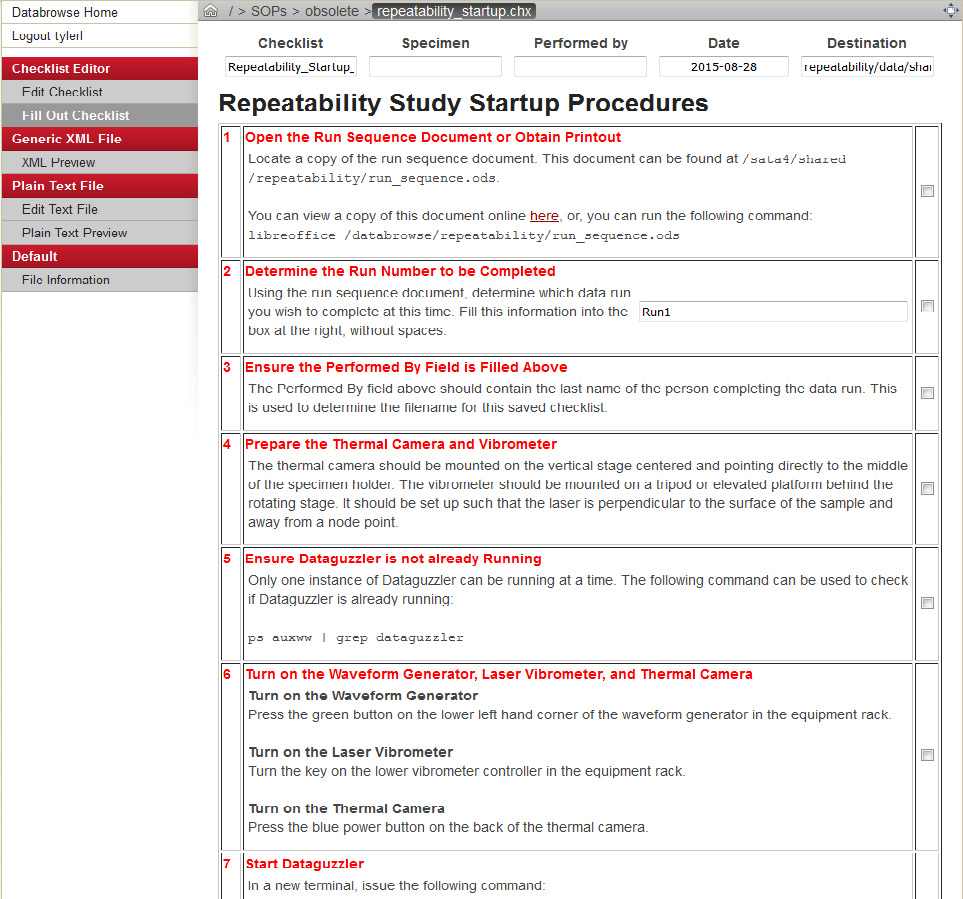
\includegraphics[width=0.45\textwidth]{Checklist_Editor.png}
\end{wrapfigure}
The checklist editor plugin is one of several Databrowse plugins that were constructed to create and modify data.  Checklists (*.chx for checklist templates and *.chf for filled checklists) are XML files that contain the necessary information to document laboratory procedures.  The complete details of the file format are outside of the scope of this document.  However, this plugin enables the user to open a checklist template, fill out a checklist, and save the filled checklist to the file system.

An experimental tool for modifying a checklist is being developed as well.  This tool utilizes the Axel XML JavaScript library (\url{http://ssire.github.io/axel/}) to provide an interface for editing the file in the web browser.

This plugin is not intended to be used from within the Databrowse library interface.

\endgroup

\hfill\break

\begingroup
\setlength\intextsep{0pt}
\subsection{Checklist Viewer}
\begin{wrapfigure}[20]{R}{0.45\textwidth}
		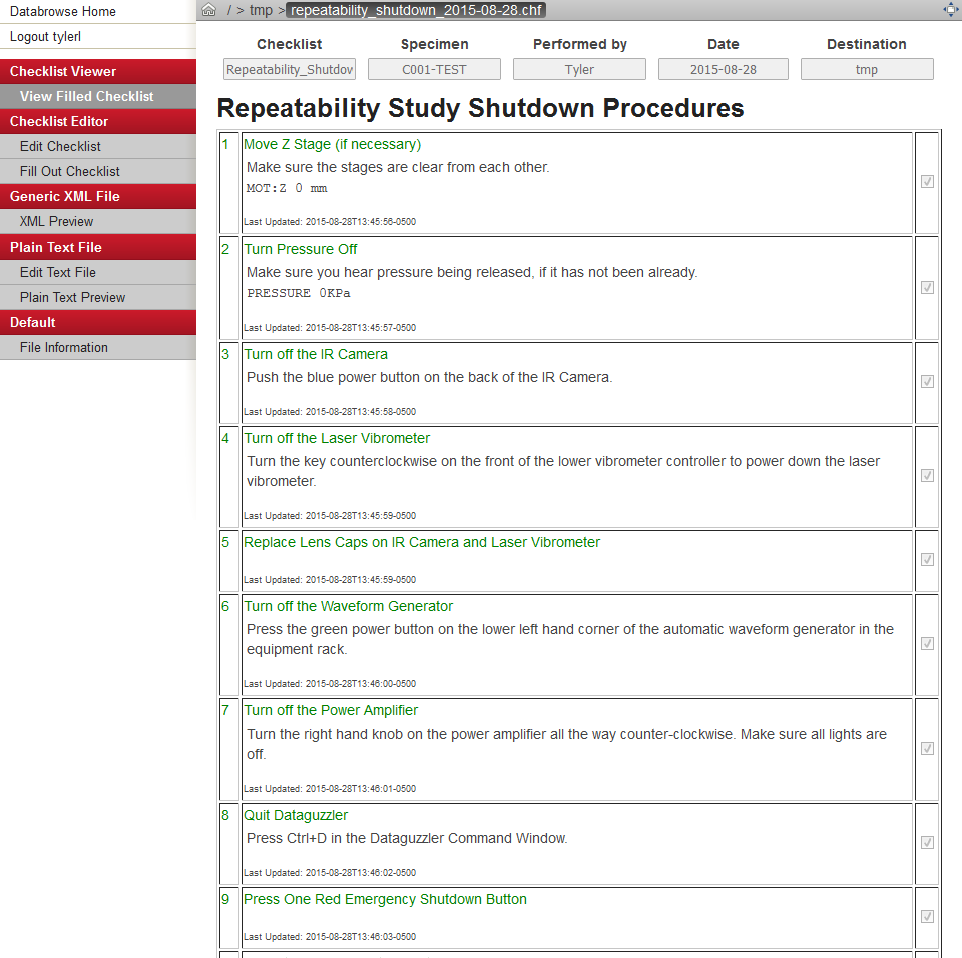
\includegraphics[width=0.45\textwidth]{Checklist_Viewer.png}
\end{wrapfigure}
The checklist viewer plugin displays filled checklist files (*.chf).  Checklists (*.chx for checklist templates and *.chf for filled checklists) are XML files that contain the necessary information to document laboratory procedures.  The complete details of the file format are outside of the scope of this document.  However, this plugin will display the status of all checklist items, along with displaying time stamp information and notes.

\endgroup

\clearpage
\begingroup
\setlength\intextsep{0pt}
\subsection{Datacollect v1 Viewer}
\begin{wrapfigure}[20]{R}{0.45\textwidth}
		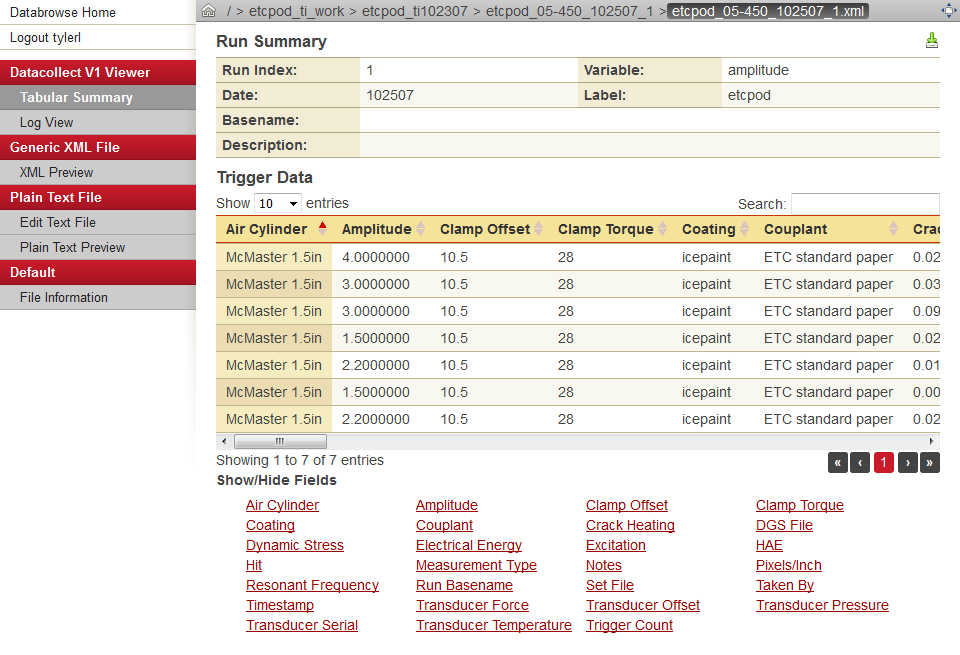
\includegraphics[width=0.45\textwidth]{Datacollect_v1_Viewer.png}
\end{wrapfigure}
Datacollect is a tool that enables the automation of data collection processes.  Version 1 of Datacollect provides an interface for the entry of experimental parameters and an interface to aid in automating use of data acquisition tools.  This plugin is responsible for displaying the data saved by Datacollect in a meaningful fashion.  It can display data in both a log-style format and in a tabular form, capable of being sorted, filtered, and searched.

\endgroup

\hfill\break
\hfill\break

\begingroup
\setlength\intextsep{0pt}
\subsection{Datacollect v2 Viewer}
\begin{wrapfigure}[20]{R}{0.45\textwidth}
		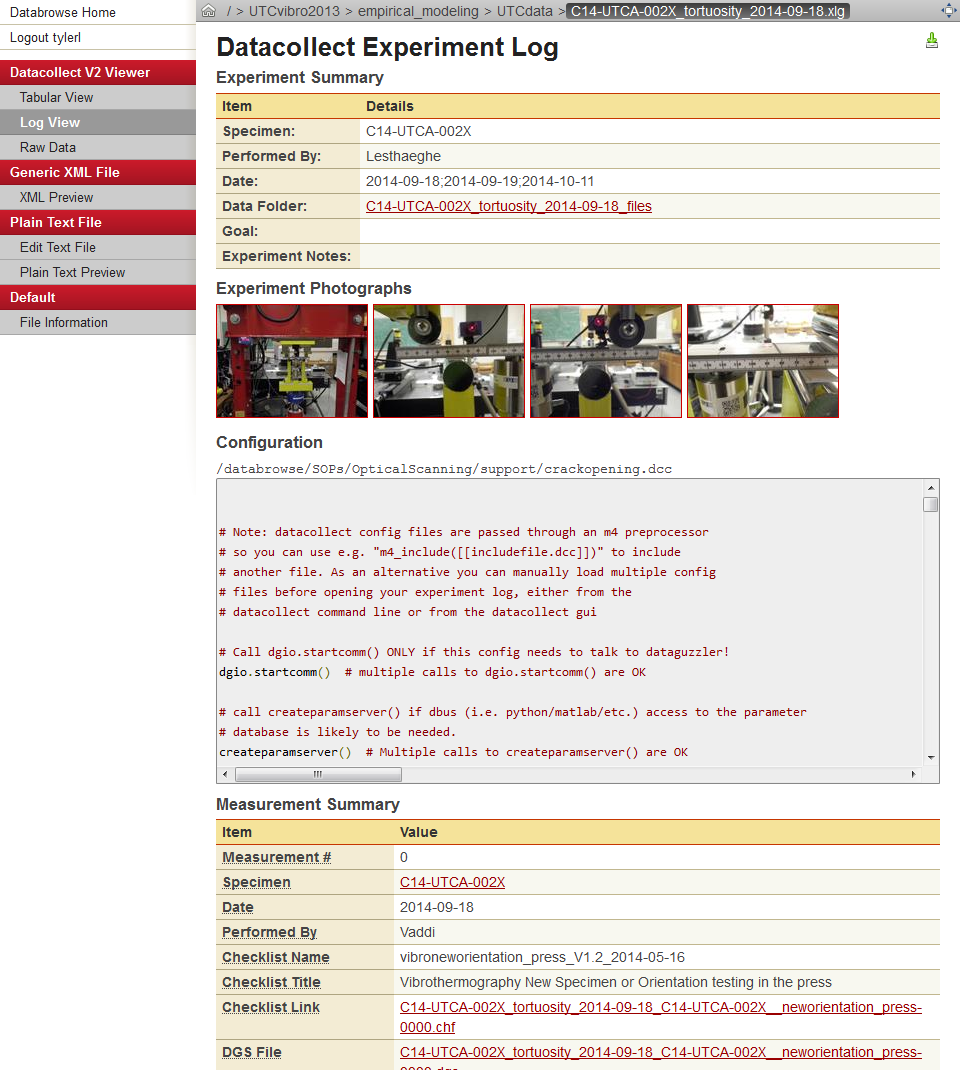
\includegraphics[width=0.45\textwidth]{Datacollect_v2_Viewer.png}
\end{wrapfigure}
Datacollect is a tool that enables the automation of data collection processes.  Version 2 of Datacollect provides an interface for the entry of experimental parameters, an interface to aid in automating use of data acquisition tools, and an interface for managing experimental processes and procedures.  This plugin is responsible for displaying the data saved by Datacollect in a meaningful fashion.  It can display data in both a log-style format and in a tabular form, capable of being sorted, filtered, and searched.

\endgroup

\hfill \break
\hfill \break
\hfill \break
\hfill \break
\hfill \break
\hfill \break
\hfill \break
\hfill \break
\hfill \break

\begingroup
\setlength\intextsep{0pt}
\subsection{Dataguzzler Data File}
\begin{wrapfigure}[20]{R}{0.45\textwidth}
		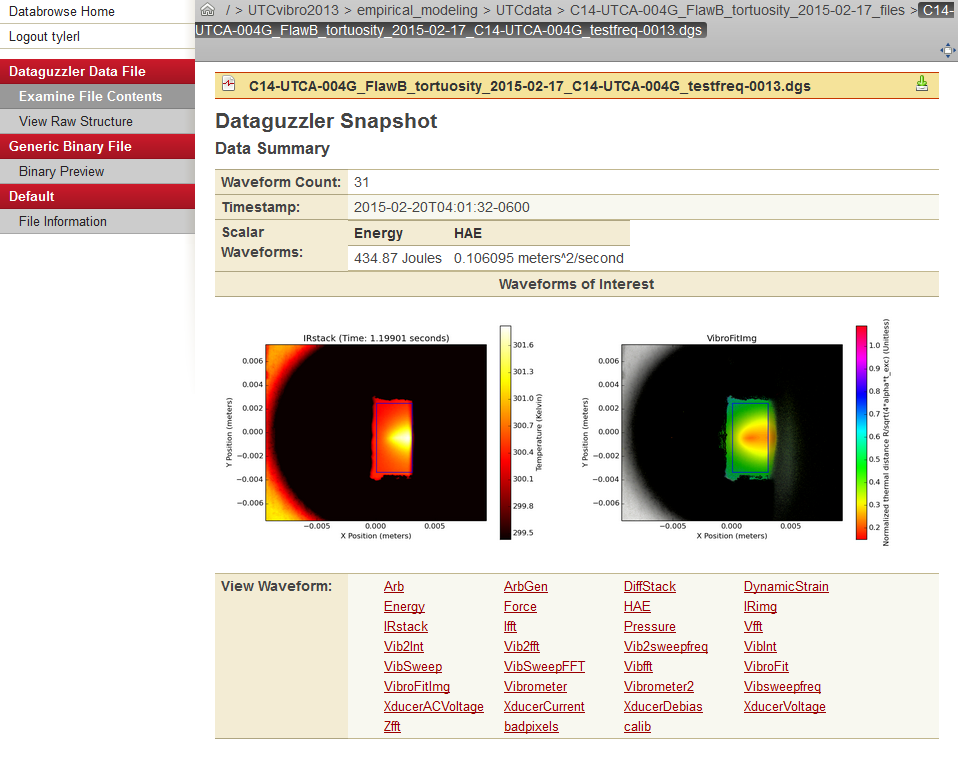
\includegraphics[width=0.45\textwidth]{Dataguzzler_DGS_File.png}
\end{wrapfigure}
Dataguzzler is an open source extensible data acquisition platform -- providing a high speed mechanism for data capture, storage, and visualization.  Dataguzzler also provides bindings enabling simple integration with data collection automation scripts and other related programs.  The Dataguzzler data file plugin for Databrowse enables the user to view the data contained within Dataguzzler binary data files (*.dgs, *.dgd, *.dga, *.dgz).  The plugin utilizes Matplotlib for Python to produce realtime visualizations of data, in addition to displaying all of the associated meta data.  The plugin can also export data from Dataguzzler data files into several other common file formats, including CSV and MAT.  The plugin is also capable of exporting videos from the appropriate types of data.

\endgroup


\clearpage
\begingroup
\setlength\intextsep{0pt}
\subsection{Dataguzzler Settings File}
\begin{wrapfigure}[20]{R}{0.45\textwidth}
		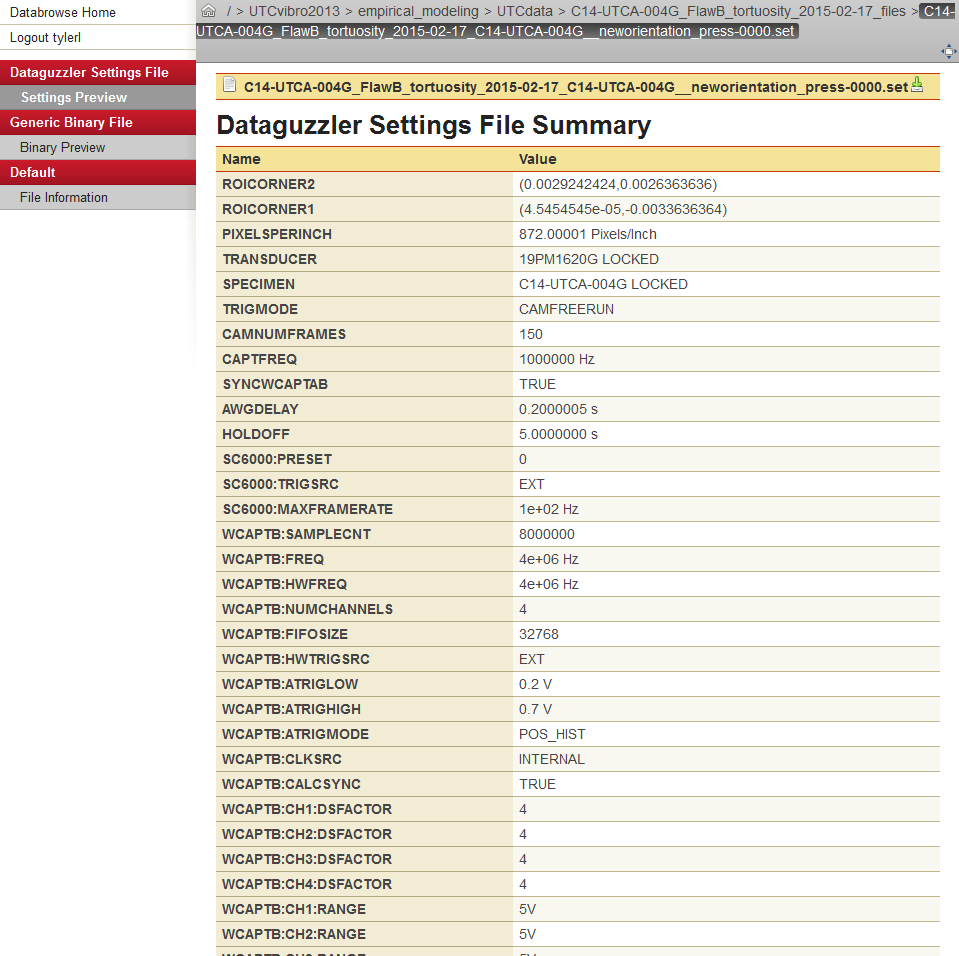
\includegraphics[width=0.45\textwidth]{Dataguzzler_SET_File.png}
\end{wrapfigure}
Dataguzzler is an open source extensible data acquisition platform -- providing a high speed mechanism for data capture, storage, and visualization.  Dataguzzler also provides bindings enabling simple integration with data collection automation scripts and other related programs.  The Dataguzzler set file plugin for Databrowse enables the user to examine the contents of Dataguzzler settings files (*.set).

\endgroup

\hfill \break
\hfill \break
\hfill \break
\hfill \break
\hfill \break
\hfill \break
\hfill \break
\hfill \break

\begingroup
\setlength\intextsep{0pt}
\subsection{Data Table}
\begin{wrapfigure}[20]{R}{0.45\textwidth}
		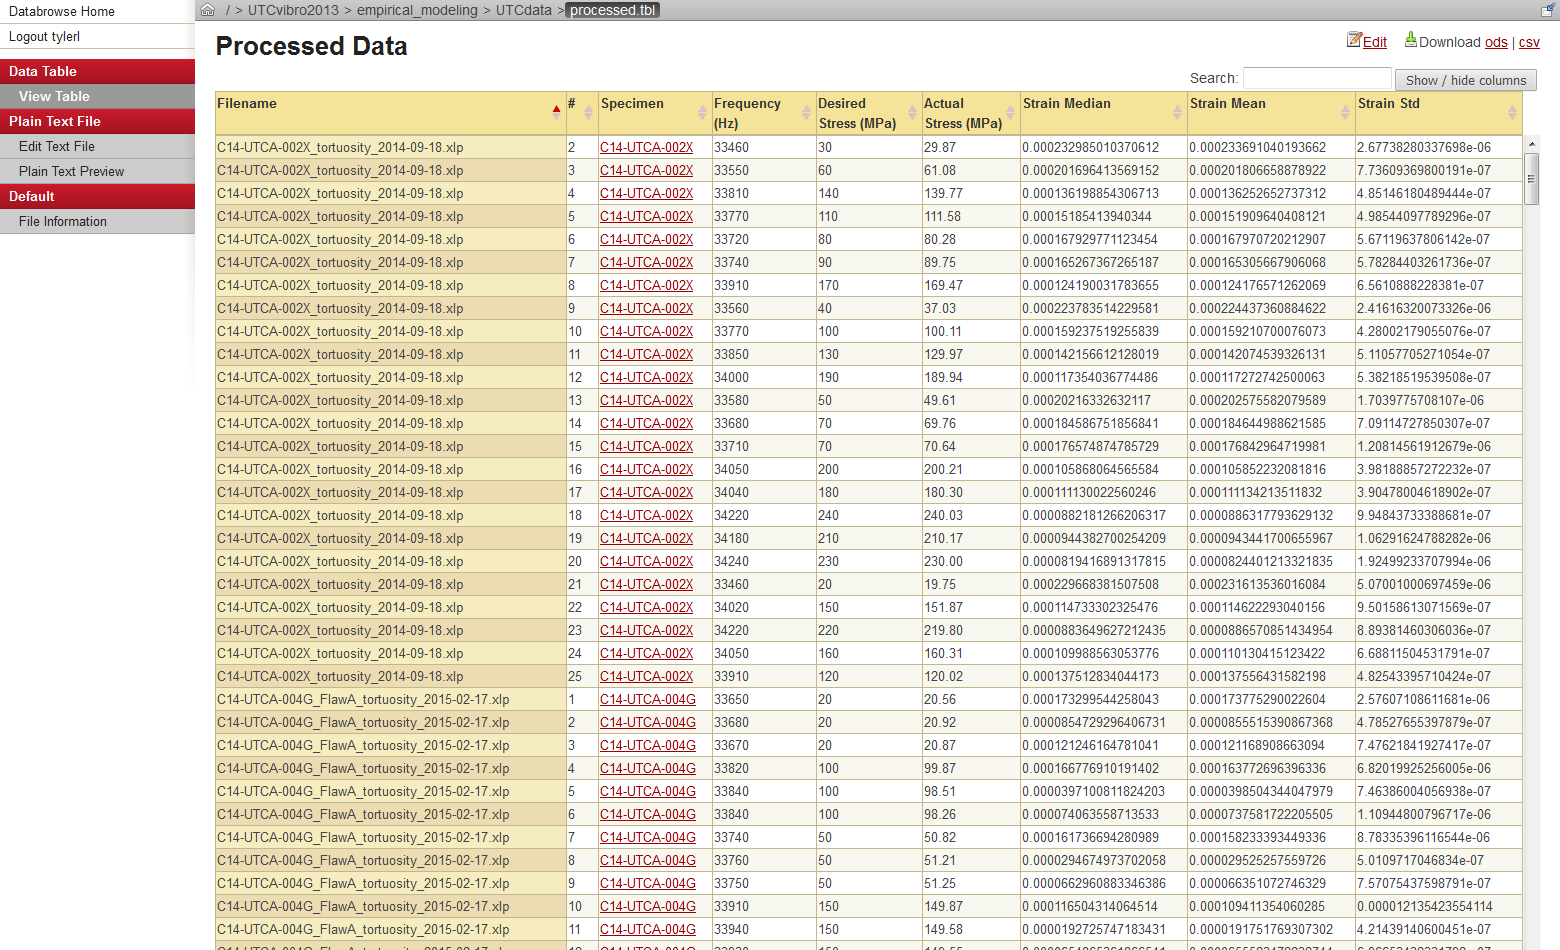
\includegraphics[width=0.45\textwidth]{Data_Table.png}
\end{wrapfigure}
The data table plugin is a tool designed to aid in the collection and compilation of large data sets from multiple sources.  This plugin operates on *.tbl files.  The exact schema of the *.tbl file is outside of the scope of this document; however, the tbl file is an XML file which instructs the Data Table plugin where to find data files and how to select data from them.  The end result is a new XML document that combines all of this data together.  This XML document can then be rendered by Databrowse in the web browser in the form of a searchable, sortable, and filterable table.  This table can be exported to CSV from the web browser as well.  Additionally, this plugin can prove to be very powerful when utilized inside of a processing script using the Databrowse library, enabling rapid development of data processing scripts that can operate on large sets of data in real time.  

\endgroup


\begingroup
\setlength\intextsep{0pt}
\subsection{Default}
\begin{wrapfigure}[20]{R}{0.45\textwidth}
		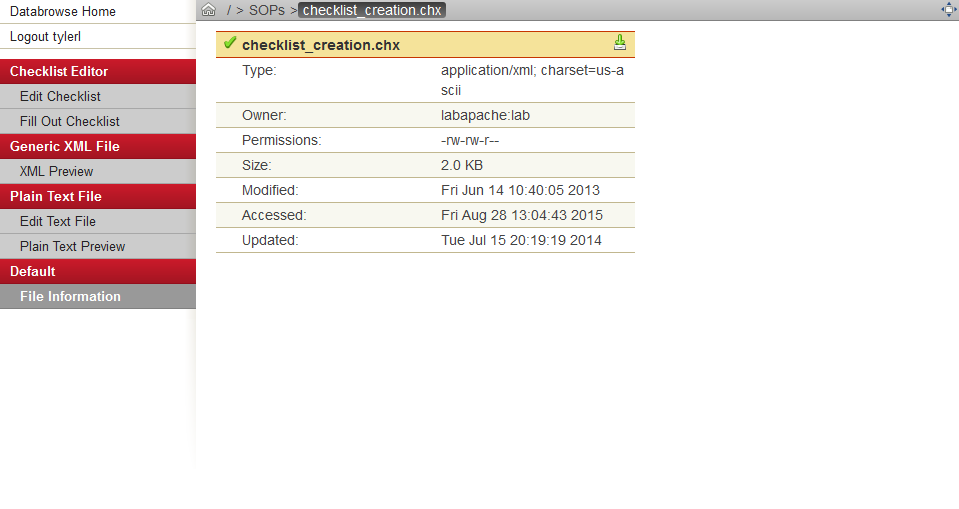
\includegraphics[width=0.45\textwidth]{Default_Plugin.png}
\end{wrapfigure}
The default plugin is a catch-all plugin that can operate on any type of file.  This ensures that even for files in which Databrowse is unable to determine the appropriate plugin to use, or a plugin does not exist that supports a particular file type, some set of information about the file can be returned and displayed.  This plugin will extract basic file information, such as file name, size, timestamps, and permissions.

\endgroup


\clearpage
\begingroup
\setlength\intextsep{0pt}
\subsection{Directory}
\begin{wrapfigure}[20]{R}{0.45\textwidth}
		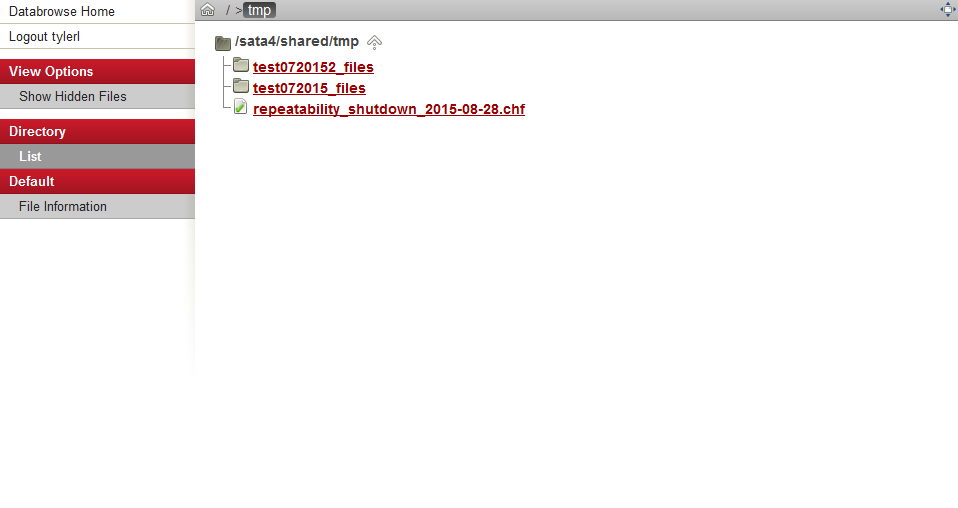
\includegraphics[width=0.45\textwidth]{Directory.png}
\end{wrapfigure}
The generic directory plugin is capable of scanning a folder and building an XML representation of the contents of that folder.  It is also capable of recursively building a representation of entire directory trees.  In the web interface, this is displayed as the default file browser view.  The web browser interface has a number of useful features that enable the user to perform operations on files.  See Section \ref{GettingStarted} for additional information about this interface.

\endgroup



\begin{changemargin}{0in}{220.6pt}
\subsection{File Operations}
The file operations plugin is a special plugin that is normally not visible from the web or library interface.  This plugin enables other plugins to perform special operations on files, particularly those that do not yet exist.
\end{changemargin}



\begingroup
\setlength\intextsep{0pt}
\subsection{Generic Binary File}
\begin{wrapfigure}[20]{R}{0.45\textwidth}
		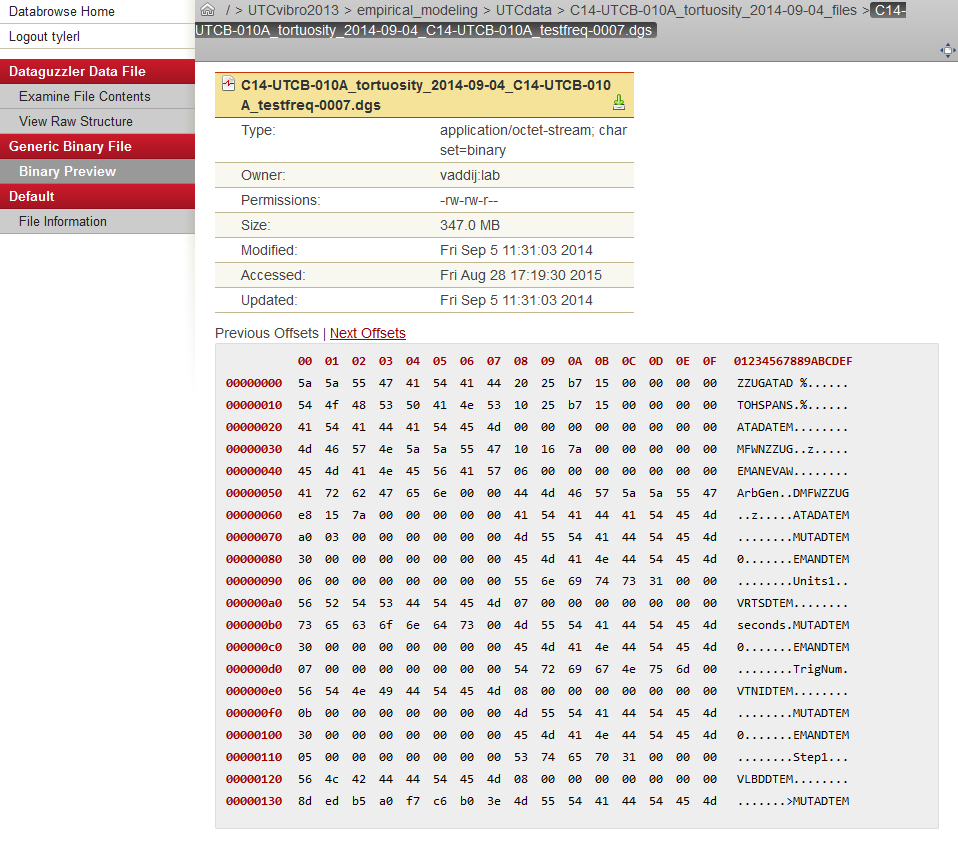
\includegraphics[width=0.45\textwidth]{Generic_Binary_File.png}
\end{wrapfigure}
The generic binary file plugin is capable of reading out data in a hex and ASCII format from a binary data file.  In the web interface, generic information is displayed about the file, along with an interactive hex viewer tool.  The viewer will only pull in a small chunk of the file at a time, since binary files can be rather large.  AJAX requests are made by the web browser enabling the user to browse through the file interactively in real time.

\endgroup

\clearpage
\begingroup
\setlength\intextsep{0pt}
\subsection{Generic HDF5 File}
\begin{wrapfigure}[20]{R}{0.45\textwidth}
		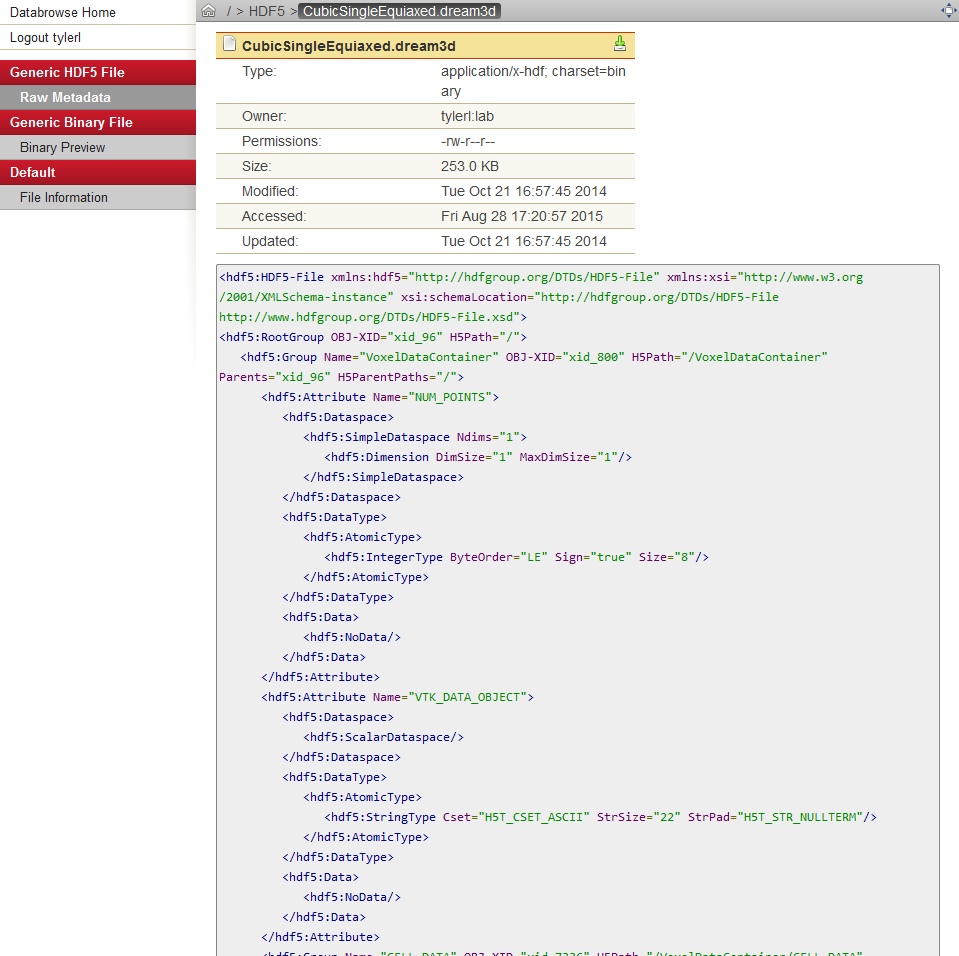
\includegraphics[width=0.45\textwidth]{Generic_HDF5_File.png}
\end{wrapfigure}
The HDF5 viewer plugin is a work-in-progress plugin that will simply display the internal structure of an HDF5 file at this time.

\endgroup

\hfill \break
\hfill \break
\hfill \break
\hfill \break
\hfill \break
\hfill \break
\hfill \break
\hfill \break
\hfill \break
\hfill \break
\hfill \break
\hfill \break
\hfill \break


\begin{changemargin}{0in}{220.6pt}
\subsection{Generic WSGI Application}
The generic WSGI application plugin will enable a WSGI compliant Python script to be ran inside the context of Databrowse.  This is very useful for scenarios in which an end user wishes to quickly create an interactive web application within the context of a particular set of data or for a task-oriented purpose without the need to create an infrastructure in which that application will run.
\end{changemargin}


\begingroup
\setlength\intextsep{0pt}
\subsection{Generic XML File}
\begin{wrapfigure}[20]{R}{0.45\textwidth}
		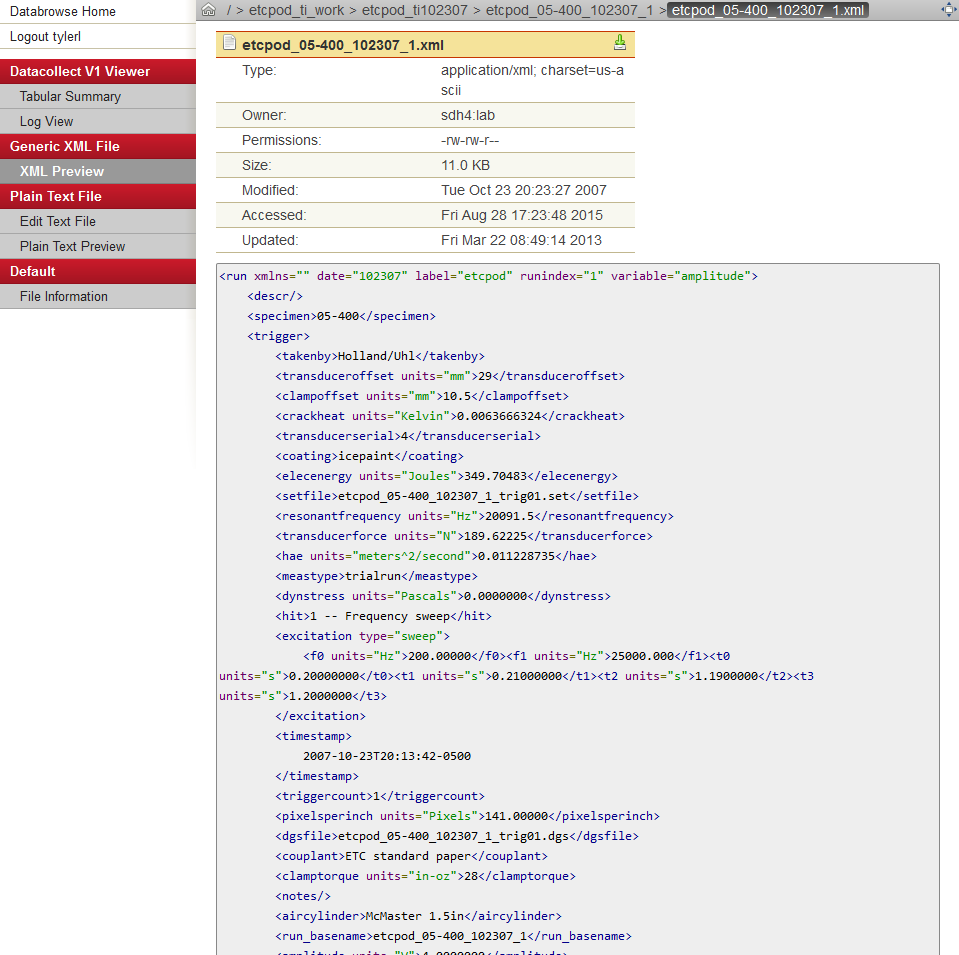
\includegraphics[width=0.45\textwidth]{Generic_XML_File.png}
\end{wrapfigure}
The generic XML file viewer will display a textual view of an XML file, along with basic file information.

\endgroup

\clearpage
\begingroup
\setlength\intextsep{0pt}
\subsection{Image Viewer}
\begin{wrapfigure}[20]{R}{0.45\textwidth}
		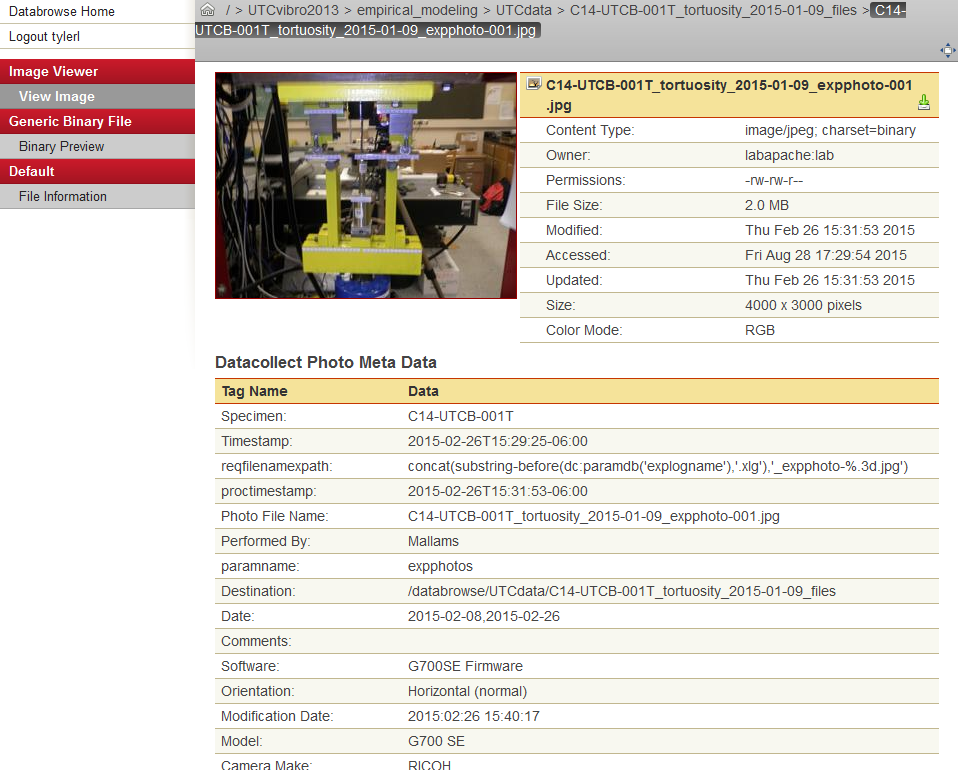
\includegraphics[width=0.45\textwidth]{Image_Viewer.png}
\end{wrapfigure}
The image viewer plugin will display an image, in addition to all internal metadata and EXIF tags associated with an image.  The plugin also supports the ability to resize images in real time for use by other plugins as well.  It will operate on any file type supported by the Python Imaging Library, including *.png, *.jpg, *.bmp, and many more.

\endgroup

\hfill \break
\hfill \break
\hfill \break
\hfill \break
\hfill \break
\hfill \break
\hfill \break

\begingroup
\setlength\intextsep{0pt}
\subsection{Mercurial Repository}
\begin{wrapfigure}[20]{R}{0.45\textwidth}
		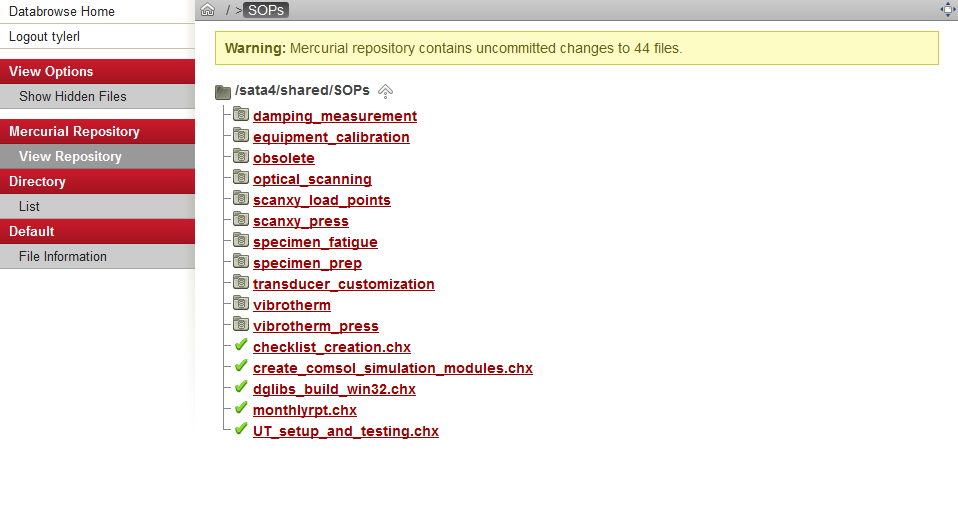
\includegraphics[width=0.45\textwidth]{Mercurial_Repository.png}
\end{wrapfigure}
Mercurial is a version tracking tool.  The Mercurial Repository Databrowse plugin is a work-in-progress that will display warning information to users about uncommitted changes and other potential concerns associated with a Mercurial repository.  This plugin overrides the default Directory plugin, though, all other functionality available from the directory plugin is still available in this context.

\endgroup

\hfill \break

\begingroup
\setlength\intextsep{0pt}
\subsection{Movie Viewer}
\begin{wrapfigure}[20]{R}{0.45\textwidth}
		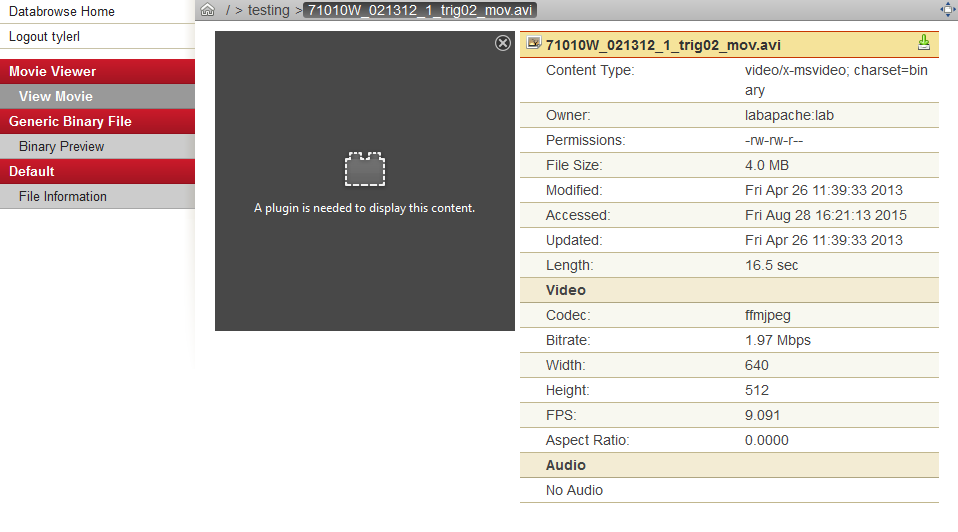
\includegraphics[width=0.45\textwidth]{Movie_Viewer.png}
\end{wrapfigure}
The movie viewer plugin is an experimental plugin that will attempt to stream video content to the users web browser.  This requires the usage of the appropriate plugins and codecs on the end user computer.  This plugin is also capable of extracting preview frames from videos.  It will operate on any video format supported by FFMPEG.

\endgroup

\clearpage
\begingroup
\setlength\intextsep{0pt}
\subsection{Multimedia Directory}
\begin{wrapfigure}[20]{R}{0.45\textwidth}
		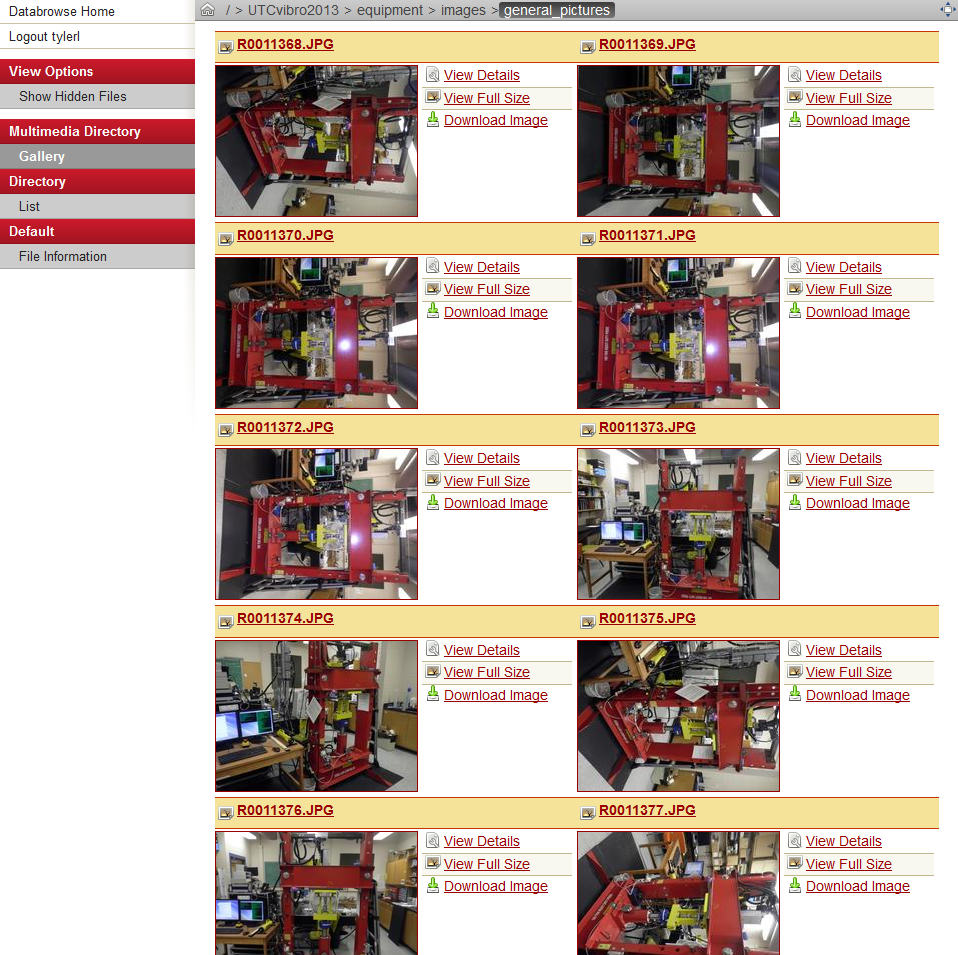
\includegraphics[width=0.45\textwidth]{Multimedia_Directory.png}
\end{wrapfigure}
The multimedia directory plugin will display thumbnail previews of image, video, and other multimedia content.  It will override the default directory plugin when the majority of the content inside of a folder can be displayed with a thumbnail preview.  Clicking on a thumbnail in the multimedia directory plugin will display a larger version of the image without leaving the page. 

\endgroup

\hfill \break
\hfill \break
\hfill \break
\hfill \break
\hfill \break
\hfill \break
\hfill \break
\hfill \break
\hfill \break
\hfill \break

\begingroup
\setlength\intextsep{0pt}
\subsection{Office Viewer}
\begin{wrapfigure}[20]{R}{0.45\textwidth}
		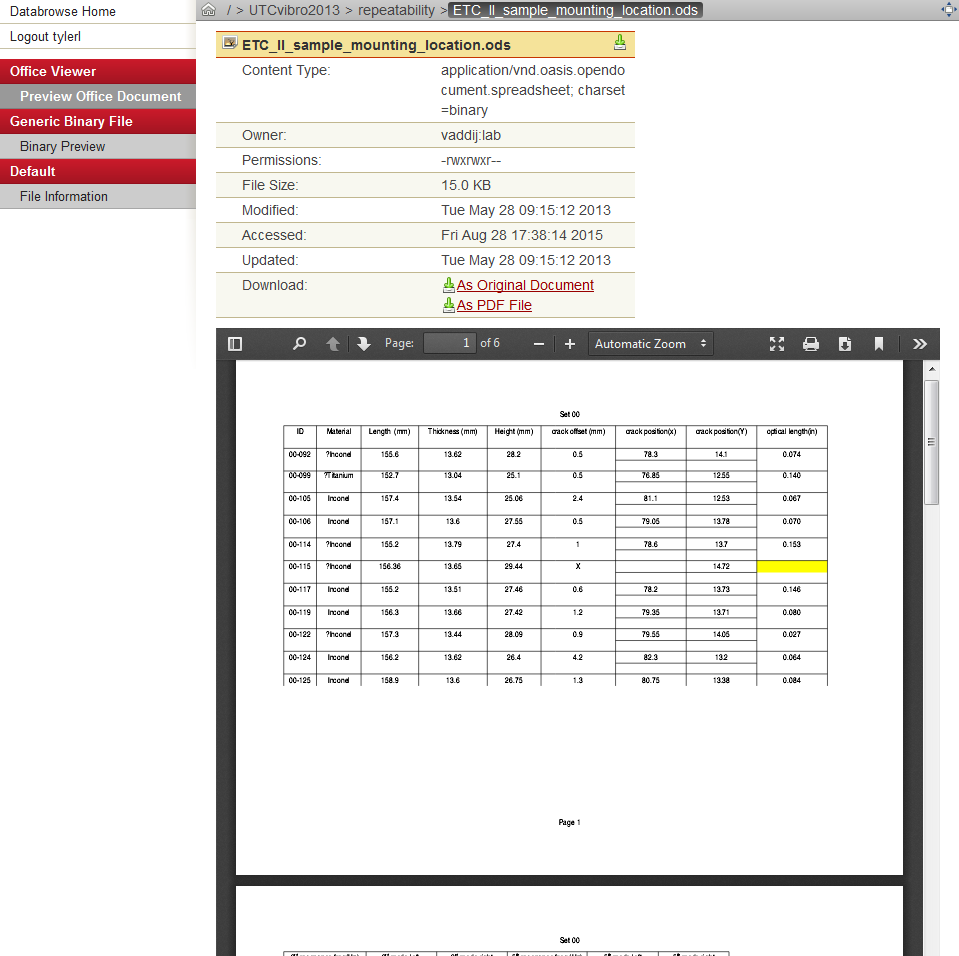
\includegraphics[width=0.45\textwidth]{Office_Viewer.png}
\end{wrapfigure}
The office viewer plugin provides an in-browser PDF preview of word processor documents, spreadsheets, presentations, and other document files.  This plugin operates on any file format supported by LibreOffice, including *.doc, *.ppt, *.xls, *.odt, *.odp, *.ods, and many others.

\endgroup

\clearpage
\begingroup
\setlength\intextsep{0pt}
\subsection{PDF Viewer}
\begin{wrapfigure}[20]{R}{0.45\textwidth}
		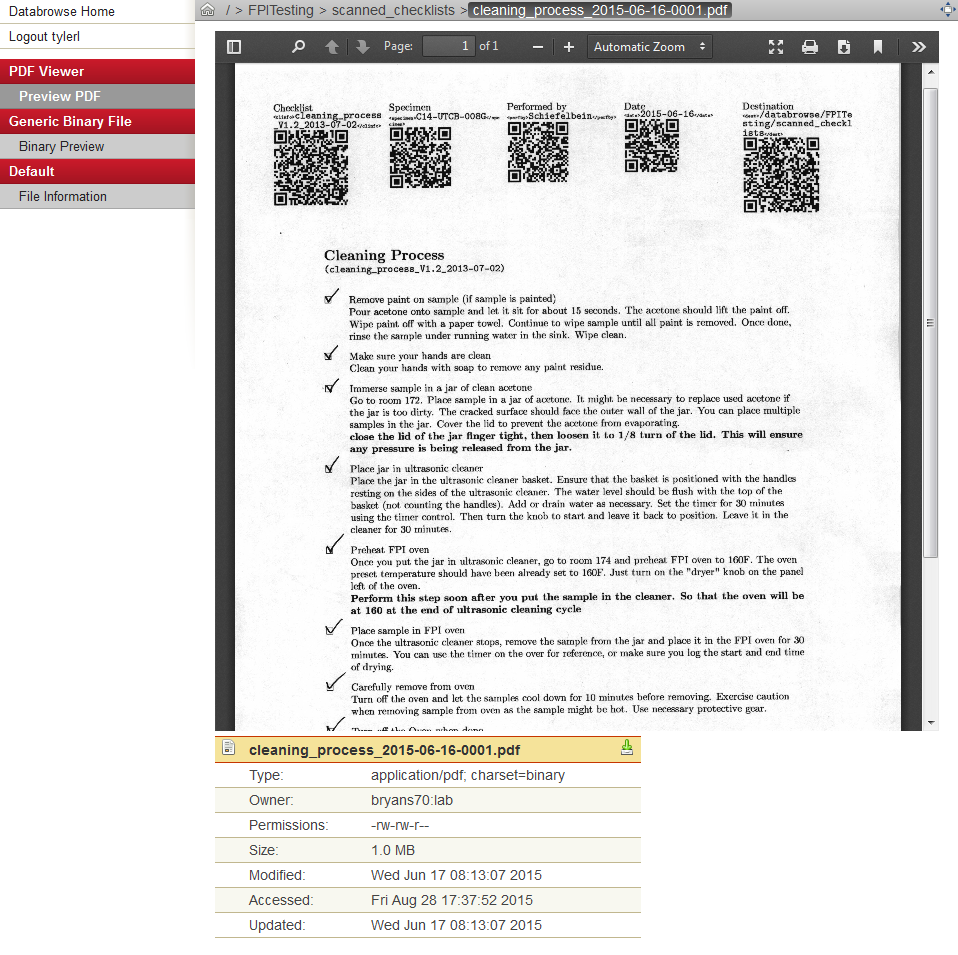
\includegraphics[width=0.45\textwidth]{PDF_Viewer.png}
\end{wrapfigure}
The PDF viewer plugin will display a PDF file for the user inside the web browser.

\endgroup

\hfill \break
\hfill \break
\hfill \break
\hfill \break
\hfill \break
\hfill \break
\hfill \break
\hfill \break
\hfill \break
\hfill \break
\hfill \break
\hfill \break
\hfill \break
\hfill \break

\begingroup
\setlength\intextsep{0pt}
\subsection{Plain Text File}
\begin{wrapfigure}[20]{R}{0.45\textwidth}
		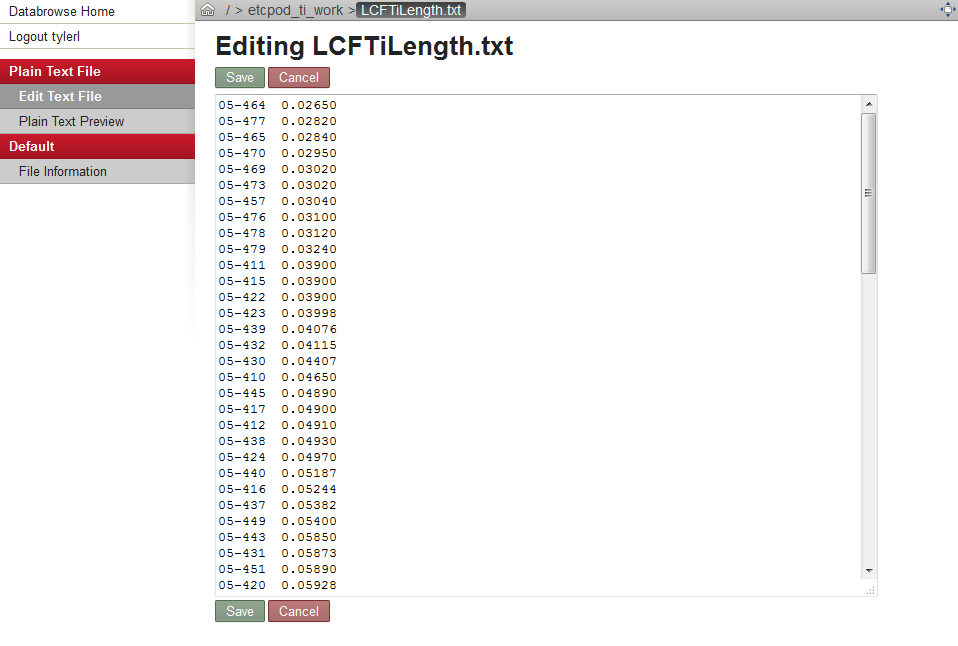
\includegraphics[width=0.45\textwidth]{Plain_Text_File.png}
\end{wrapfigure}
The plain text file plugin displays the contents of any plain text file inside the web browser.  It also provides a convenient interface for editing plain text files right in the web browser.  Backups will automatically be saved by this plugin during a save operation.  It will operate on all files with the content-type of plain/text.

\endgroup

\hfill \break
\hfill \break
\hfill \break
\hfill \break
\hfill \break

\begingroup
\setlength\intextsep{0pt}
\subsection{SolidWorks Viewer}
\begin{wrapfigure}[20]{R}{0.45\textwidth}
		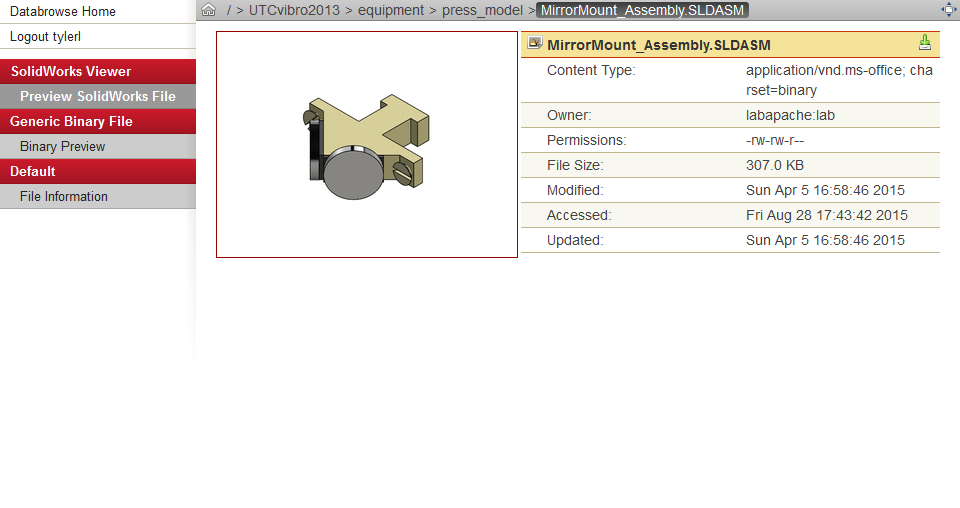
\includegraphics[width=0.45\textwidth]{SolidWorks_Viewer.png}
\end{wrapfigure}
The SolidWorks viewer plugin provides a quick low resolution image preview of a SolidWorks file in the web browser.  This plugin is also capable of providing a thumbnail for use in the context of the multimedia directory plugin and other plugins where appropriate.  It operates on files with the *.sldprt, *.sldasm, and *.slddrw extensions.

\endgroup


\clearpage
\begingroup
\setlength\intextsep{0pt}
\subsection{Specimen Management Plugin}
\begin{wrapfigure}[20]{R}{0.45\textwidth}
		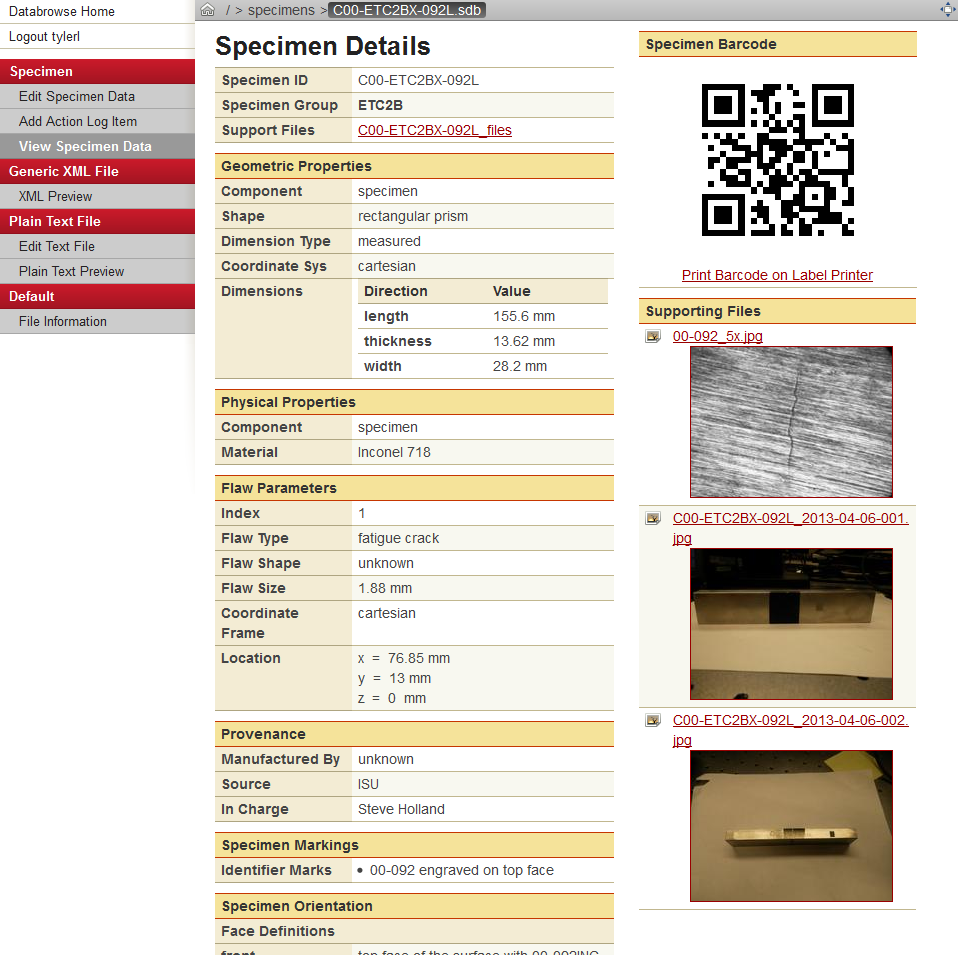
\includegraphics[width=0.45\textwidth]{Specimen_Plugin.png}
\end{wrapfigure}
The Specimen Management plugin provides an interface for storing and tracking information about specimens.  Operating on XML files containing the *.sdb extension, it can produce a visual display of the details of a specimen, including identification, geometry, provenance information, images, bar code labels, etc.  Additionally, utilizing the Axel XML JavaScript library (\url{http://ssire.github.io/axel/}), this plugin can also provide a web-based interface to edit the details of a specimen on an interactive form.  The structure of the sdb files are outside of the context of this document.  Templates that control the display and editing of specimen files can be modified, enabling the introduction of new parameters.  This plugin is also capable of combining multiple sources of data about a specimen into one unified representation, highly useful both on the web and in the context of the Databrowse library.  This capability is presently being used to enable specimens to be placed into specimen groups -- sharing all of the parameters from the group and thus limiting the unnecessary repetition of data across many files.

\endgroup



\begingroup
\setlength\intextsep{0pt}
\subsection{Specimen Directory Plugin}
\begin{wrapfigure}[20]{R}{0.45\textwidth}
		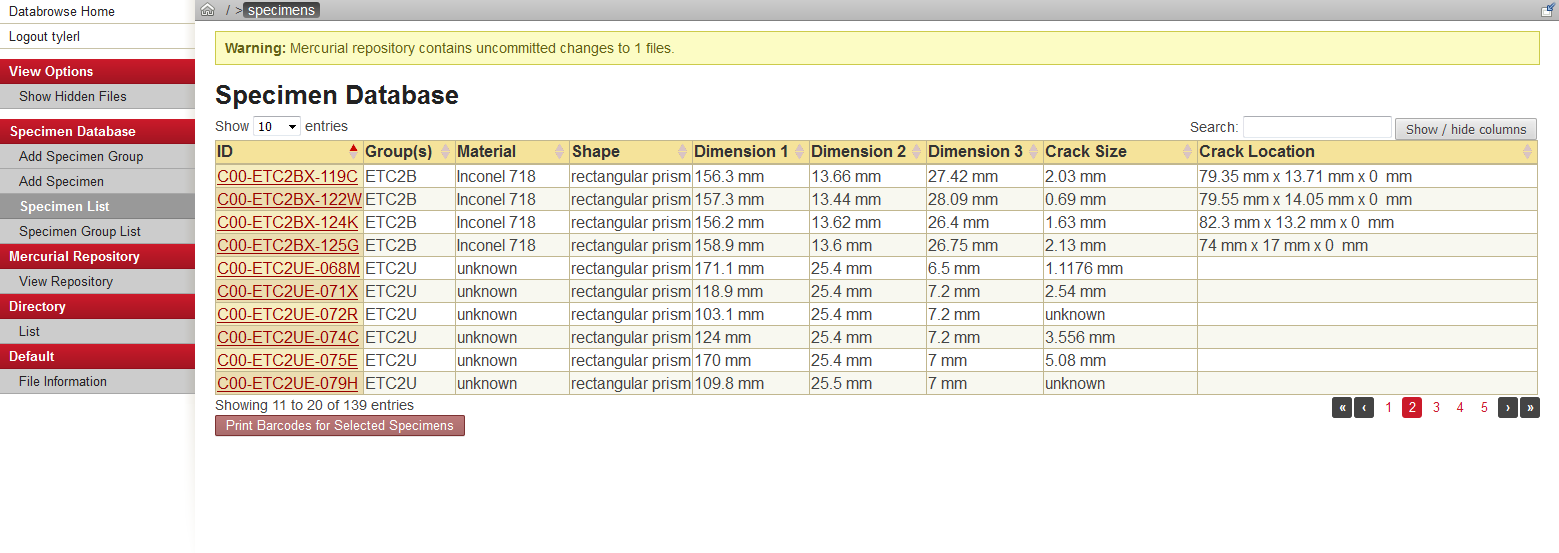
\includegraphics[width=0.45\textwidth]{Specimen_Directory_Plugin.png}
\end{wrapfigure}
The Specimen Directory plugin is a complementary tool to the Specimen Management plugin, overriding the directory plugin on directories that contain *.sdb files.  This plugin displays a tabular view of specimen parameters, enabling the quick searching, filtering, and sorting of entire sets of specimen data.  This plugin also provides easy access needed to create new *.sdb files in the current location.

\endgroup



\begingroup
\setlength\intextsep{0pt}
\subsection{Specimen Group Management Plugin}
\begin{wrapfigure}[20]{R}{0.45\textwidth}
		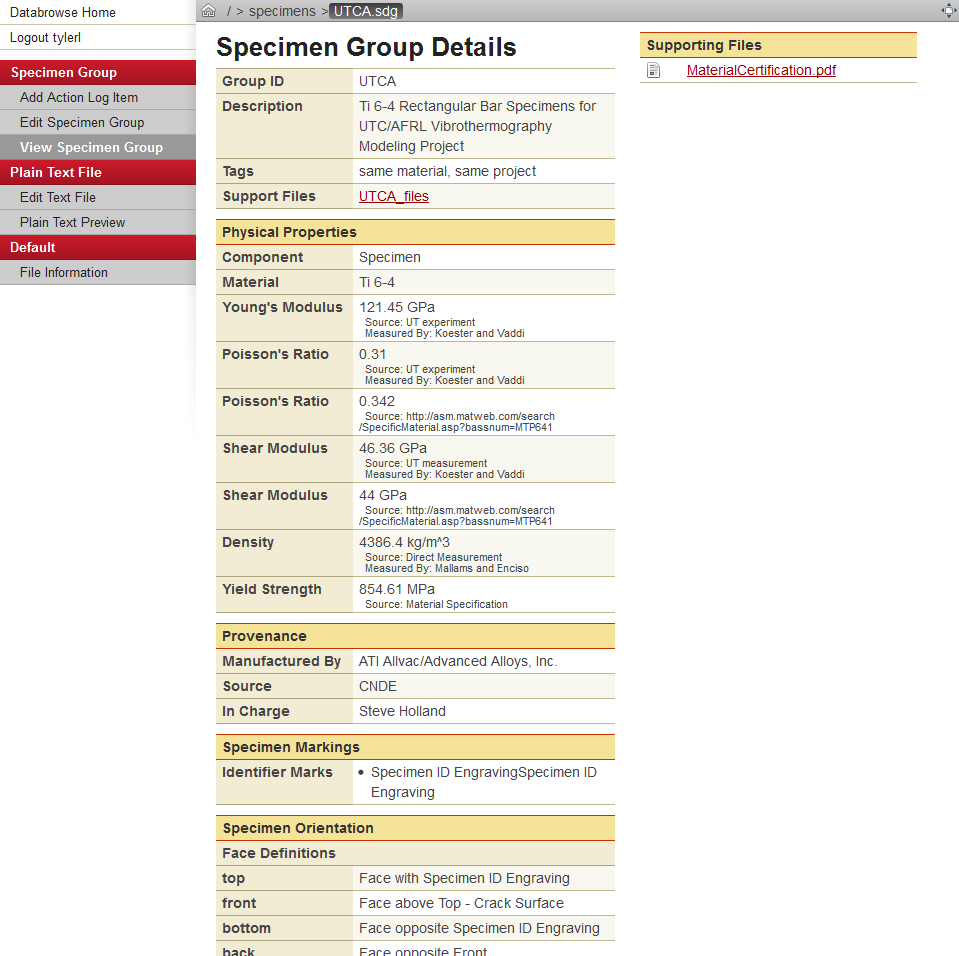
\includegraphics[width=0.45\textwidth]{Specimen_Group_Plugin.png}
\end{wrapfigure}
The Specimen Group Management plugin is a complementary tool to the Specimen Management plugin, providing similar functionality, but acting in the context of *.sdg files.  The schema defining the *.sdg file is outside of the context of this document; however, it is similar in structure to the *.sdb file.

\endgroup


\clearpage
\begingroup
\setlength\intextsep{0pt}
\subsection{SVG Viewer}
\begin{wrapfigure}[20]{R}{0.45\textwidth}
		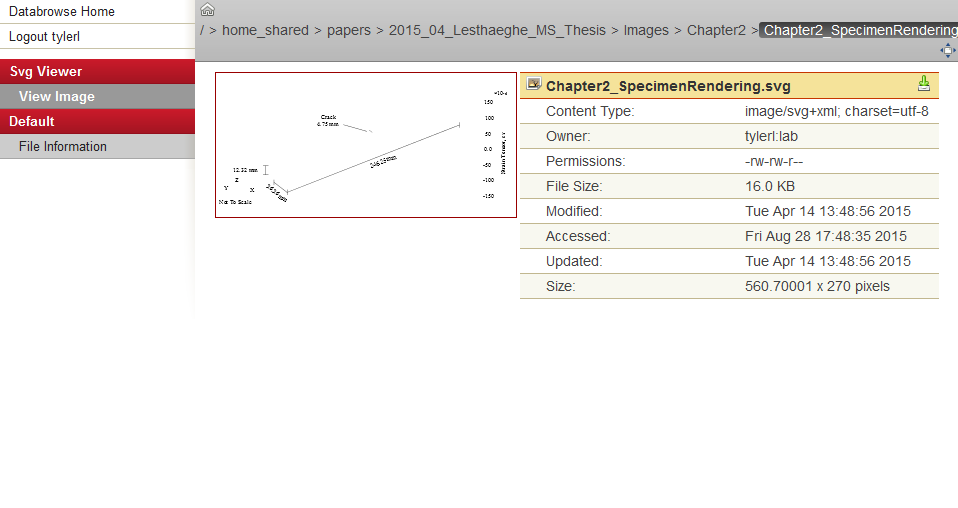
\includegraphics[width=0.45\textwidth]{SVG_Viewer.png}
\end{wrapfigure}
The SVG viewer plugin adds the necessary support to ensure that *.svg vector graphics image files can be displayed on all web browsers, producing an image thumbnail and preview if necessary.  It also produces thumbnails for the multimedia directory plugin and in other contexts as needed.

\endgroup



\begingroup
\setlength\intextsep{0pt}
\subsection{Transducer Management Plugin}
\begin{wrapfigure}[20]{R}{0.45\textwidth}
		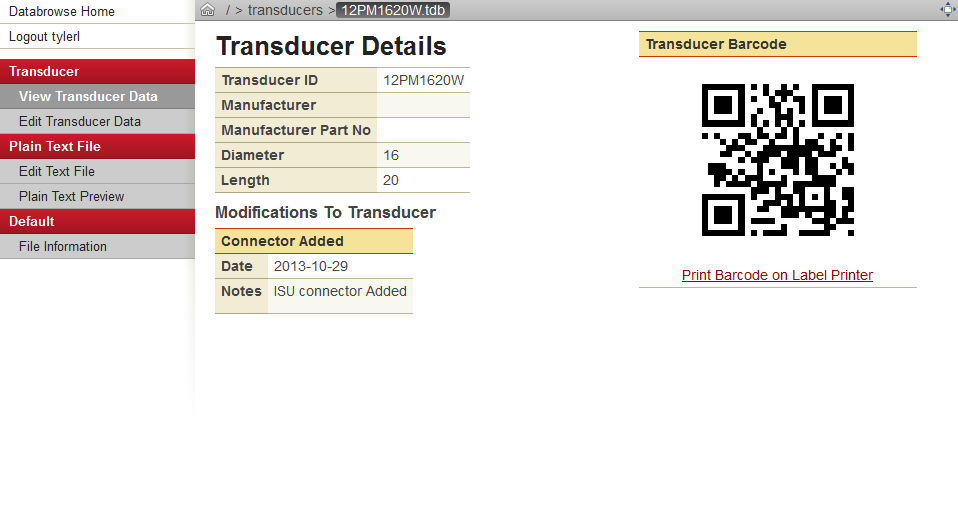
\includegraphics[width=0.45\textwidth]{Transducer_Management.png}
\end{wrapfigure}
The Transducer Management plugin is similar in functionality to the Specimen Management plugin, but designed in the context of managing parameters and other information associated with ultrasonic transducers.  The plugin operates XML files with the extension *.tdb.  The structure of these files is outside of the context of this document.

\endgroup



\begingroup
\setlength\intextsep{0pt}
\subsection{Transducer Directory Plugin}
\begin{wrapfigure}[20]{R}{0.45\textwidth}
		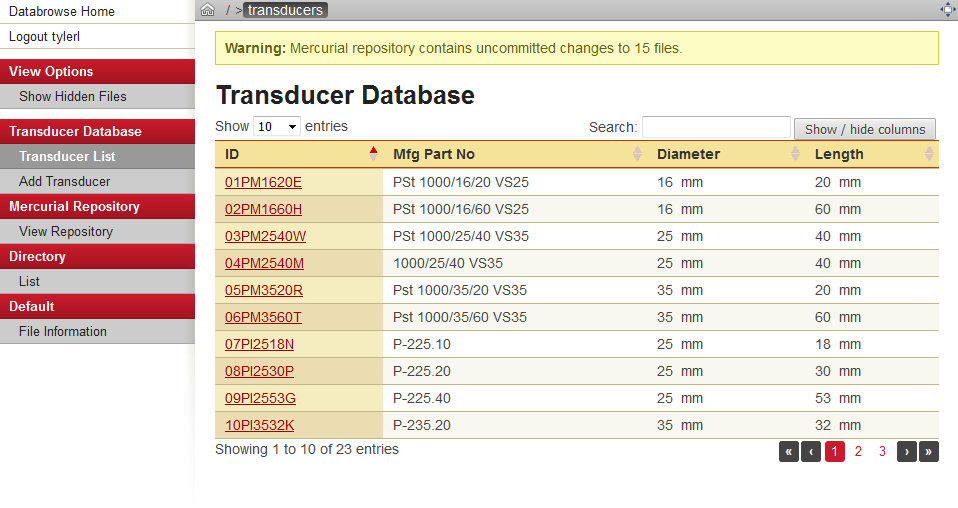
\includegraphics[width=0.45\textwidth]{Transducer_Directory_Plugin.png}
\end{wrapfigure}
The Transducer Directory plugin is similar in functionality to the Specimen Directory plugin, overriding the directory plugin on directories that contain *.tdb files, and providing a tabular view of the data contained within, enabling rapid searching, sorting, and filtering.

\endgroup

\hfill \break
\hfill \break


\begingroup
\setlength\intextsep{0pt}
\subsection{Trigger Log Plugin}
\begin{wrapfigure}[20]{R}{0.45\textwidth}
		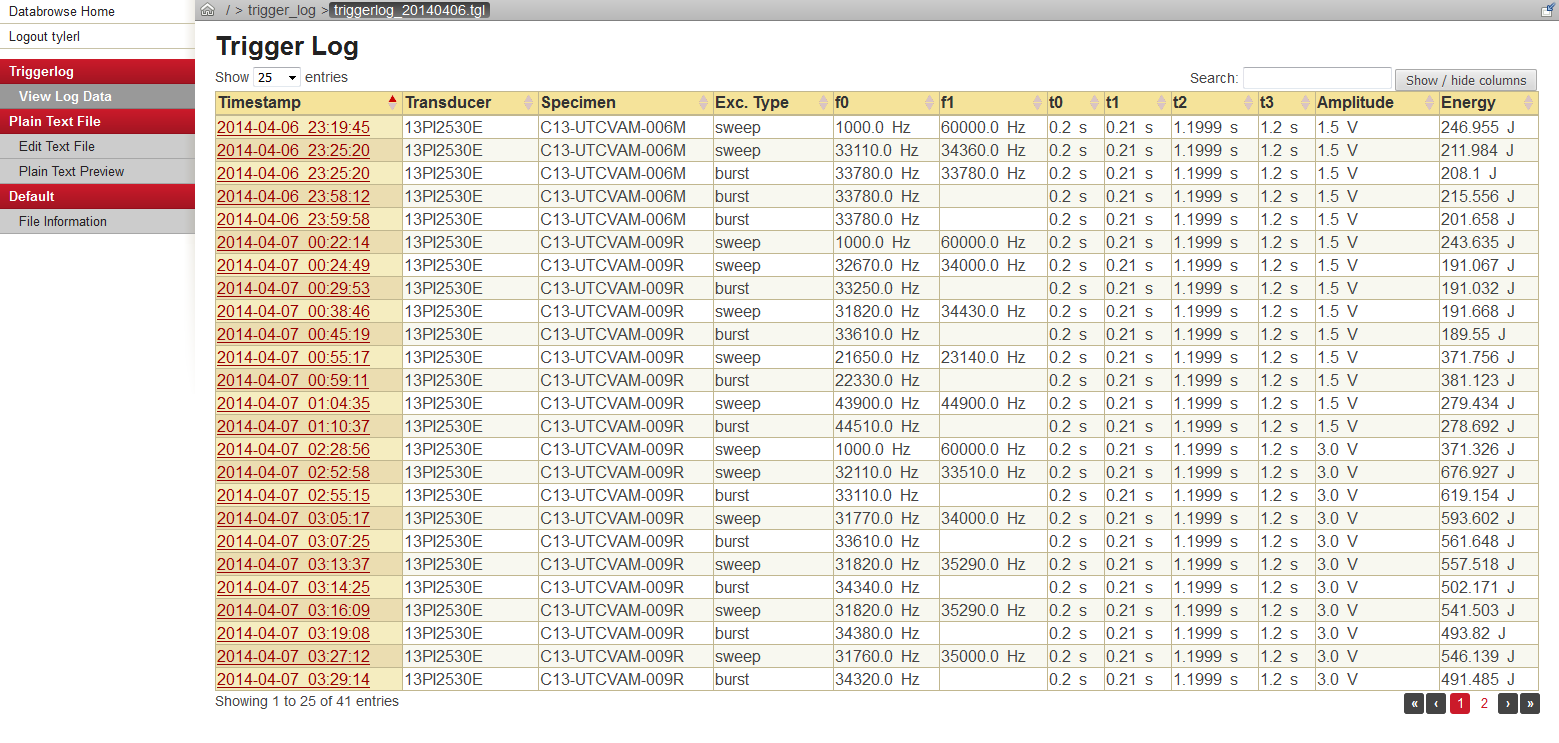
\includegraphics[width=0.45\textwidth]{Trigger_Log_Plugin.png}
\end{wrapfigure}
The Trigger Log plugin is similar in functionality to the Transducer Management plugin, but designed in the context of tracking the usage of ultrasonic transducers.  An interface with data acquisition software ensures that an XML file with the *.tgl extension is recorded to ensure accurate tracking of all experimental triggers.  This plugin will display the data from such a file in a tabular form, enabling rapid searching, sorting, and filtering.  The structure of the *.tgl file is outside of the context of this document.

\endgroup



\begingroup
\setlength\intextsep{0pt}
\subsection{Trigger Log Directory Plugin}
\begin{wrapfigure}[20]{R}{0.45\textwidth}
		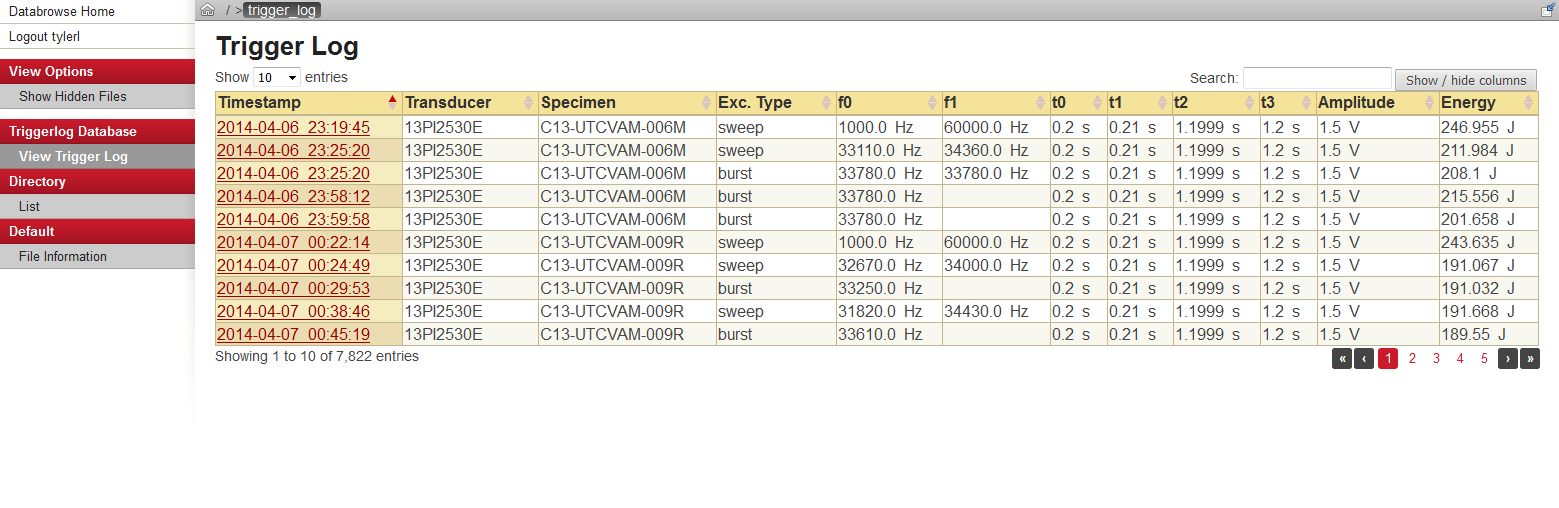
\includegraphics[width=0.45\textwidth]{Trigger_Log_Directory_Plugin.png}
\end{wrapfigure}
The Trigger Log Directory plugin functions similarly to the Trigger Log plugin, but enabling an entire directory of *.tgl files to be combined into one single representation.  This representation is displayed in tabular form, enabling rapid searching, sorting and filtering.  This plugin also provides the capability of exporting this data to a CSV file for further analysis.

\endgroup


\clearpage
\begingroup
\setlength\intextsep{0pt}
\subsection{Web Page Viewer}
\begin{wrapfigure}[20]{R}{0.45\textwidth}
		
\includegraphics[width=0.45\textwidth]{WebPage_Viewer.png}
\end{wrapfigure}
The web page viewer plugin will display the contents of an HTML file within the Databrowse interface.  Combined with the plain text editor plugin, this plugin can provide a convenient mechanism for documentation while being able to pull together all of the other resources available inside the context of Databrowse.

\endgroup

\clearpage
\section{License and Third-Party Components}
Databrowse is distributed under the terms of the BSD-3 clause license. \\

\noindent Databrowse is packaged with the following third party components: \\

\noindent Portions of this software are adapted from gnome-icon-theme-3.7.4: \\
Copyright \copyright\ 2005-2013 The GNOME Project \\
License: LGPL v3 or CC-BY-SA v3.0 \\

\noindent Portions of this software are adapted from jQuery-1.9.1: \\
Copyright \copyright\ 2013 jQuery Foundation and other contributors \\
License: MIT \\

\noindent Portions of this software are adapted from DataTables-1.9.4: \\
Copyright \copyright\ 2008-2010 Allan Jardine \\
License: GPL v2 or BSD-3 \\

\noindent Portions of this software are adapted from hurry.filesize-0.9: \\
Copyright \copyright\ 2009 Martijn Faassen, Startifact \\
License: ZPL v2.1 \\

\noindent Portions of this software are adapted from prettify-4-Mar-2013: \\
Copyright \copyright\ 2011 Mike Samuel et al \\
License: Apache v2.0 \\

\noindent Portions of this software are adapted from jQuery-File-Upload-7.4.1-jquery.ui: \\
Copyright \copyright\ 2013 Sebastian Tschan \\
License: MIT \\

\noindent Portions of this software are adapted from axel-1.1.2-beta: \\
Copyright \copyright\ 2008 - 2010 Staphane Sire \\
License: LGPL v2.1 or newer \\

\noindent Portions of this software are adapted from images2gif.py: \\
Copyright \copyright\ 2012 Almar Klein, Ant1, Marius van Voorden \\
License: BSD-3 \\


\clearpage
\subsection{BSD 3-Clause License}
Redistribution and use in source and binary forms, with or without
modification, are permitted provided that the following conditions
are met:

1. Redistributions of source code must retain the above copyright
   notice, this list of conditions and the following disclaimer.

2. Redistributions in binary form must reproduce the above copyright
   notice, this list of conditions and the following disclaimer in the
   documentation and/or other materials provided with the distribution.

3. The name of the author may not be used to endorse or promote products
   derived from this software without specific prior written permission.

THIS SOFTWARE IS PROVIDED BY THE AUTHOR ``AS IS'' AND ANY EXPRESS OR
IMPLIED WARRANTIES, INCLUDING, BUT NOT LIMITED TO, THE IMPLIED WARRANTIES
OF MERCHANTABILITY AND FITNESS FOR A PARTICULAR PURPOSE ARE DISCLAIMED.
IN NO EVENT SHALL THE AUTHOR BE LIABLE FOR ANY DIRECT, INDIRECT,
INCIDENTAL, SPECIAL, EXEMPLARY, OR CONSEQUENTIAL DAMAGES (INCLUDING, BUT
NOT LIMITED TO, PROCUREMENT OF SUBSTITUTE GOODS OR SERVICES; LOSS OF USE,
DATA, OR PROFITS; OR BUSINESS INTERRUPTION) HOWEVER CAUSED AND ON ANY
THEORY OF LIABILITY, WHETHER IN CONTRACT, STRICT LIABILITY, OR TORT
(INCLUDING NEGLIGENCE OR OTHERWISE) ARISING IN ANY WAY OUT OF THE USE OF
THIS SOFTWARE, EVEN IF ADVISED OF THE POSSIBILITY OF SUCH DAMAGE.

\clearpage
\subsection{GNU General Public License v3}
\begin{center}
{\parindent 0in
\textbf{GNU GENERAL PUBLIC LICENSE}\\
Version 3, 29 June 2007 \\

Copyright \copyright\  2007 Free Software Foundation, Inc. \texttt{http://fsf.org/}

\bigskip
Everyone is permitted to copy and distribute verbatim copies of this

license document, but changing it is not allowed.}

\end{center}

\renewcommand{\abstractname}{Preamble}
\begin{abstract}
The GNU General Public License is a free, copyleft license for
software and other kinds of works.

The licenses for most software and other practical works are designed
to take away your freedom to share and change the works.  By contrast,
the GNU General Public License is intended to guarantee your freedom to
share and change all versions of a program--to make sure it remains free
software for all its users.  We, the Free Software Foundation, use the
GNU General Public License for most of our software; it applies also to
any other work released this way by its authors.  You can apply it to
your programs, too.

When we speak of free software, we are referring to freedom, not
price.  Our General Public Licenses are designed to make sure that you
have the freedom to distribute copies of free software (and charge for
them if you wish), that you receive source code or can get it if you
want it, that you can change the software or use pieces of it in new
free programs, and that you know you can do these things.

To protect your rights, we need to prevent others from denying you
these rights or asking you to surrender the rights.  Therefore, you have
certain responsibilities if you distribute copies of the software, or if
you modify it: responsibilities to respect the freedom of others.

For example, if you distribute copies of such a program, whether
gratis or for a fee, you must pass on to the recipients the same
freedoms that you received.  You must make sure that they, too, receive
or can get the source code.  And you must show them these terms so they
know their rights.

Developers that use the GNU GPL protect your rights with two steps:
(1) assert copyright on the software, and (2) offer you this License
giving you legal permission to copy, distribute and/or modify it.

For the developers' and authors' protection, the GPL clearly explains
that there is no warranty for this free software.  For both users' and
authors' sake, the GPL requires that modified versions be marked as
changed, so that their problems will not be attributed erroneously to
authors of previous versions.

Some devices are designed to deny users access to install or run
modified versions of the software inside them, although the manufacturer
can do so.  This is fundamentally incompatible with the aim of
protecting users' freedom to change the software.  The systematic
pattern of such abuse occurs in the area of products for individuals to
use, which is precisely where it is most unacceptable.  Therefore, we
have designed this version of the GPL to prohibit the practice for those
products.  If such problems arise substantially in other domains, we
stand ready to extend this provision to those domains in future versions
of the GPL, as needed to protect the freedom of users.

Finally, every program is threatened constantly by software patents.
States should not allow patents to restrict development and use of
software on general-purpose computers, but in those that do, we wish to
avoid the special danger that patents applied to a free program could
make it effectively proprietary.  To prevent this, the GPL assures that
patents cannot be used to render the program non-free.

The precise terms and conditions for copying, distribution and
modification follow.
\end{abstract}

\begin{center}
{\Large \sc Terms and Conditions}
\end{center}


\begin{enumerate}

\addtocounter{enumi}{-1}

\item Definitions.

``This License'' refers to version 3 of the GNU General Public License.

``Copyright'' also means copyright-like laws that apply to other kinds of
works, such as semiconductor masks.

``The Program'' refers to any copyrightable work licensed under this
License.  Each licensee is addressed as ``you''.  ``Licensees'' and
``recipients'' may be individuals or organizations.

To ``modify'' a work means to copy from or adapt all or part of the work
in a fashion requiring copyright permission, other than the making of an
exact copy.  The resulting work is called a ``modified version'' of the
earlier work or a work ``based on'' the earlier work.

A ``covered work'' means either the unmodified Program or a work based
on the Program.

To ``propagate'' a work means to do anything with it that, without
permission, would make you directly or secondarily liable for
infringement under applicable copyright law, except executing it on a
computer or modifying a private copy.  Propagation includes copying,
distribution (with or without modification), making available to the
public, and in some countries other activities as well.

To ``convey'' a work means any kind of propagation that enables other
parties to make or receive copies.  Mere interaction with a user through
a computer network, with no transfer of a copy, is not conveying.

An interactive user interface displays ``Appropriate Legal Notices''
to the extent that it includes a convenient and prominently visible
feature that (1) displays an appropriate copyright notice, and (2)
tells the user that there is no warranty for the work (except to the
extent that warranties are provided), that licensees may convey the
work under this License, and how to view a copy of this License.  If
the interface presents a list of user commands or options, such as a
menu, a prominent item in the list meets this criterion.

\item Source Code.

The ``source code'' for a work means the preferred form of the work
for making modifications to it.  ``Object code'' means any non-source
form of a work.

A ``Standard Interface'' means an interface that either is an official
standard defined by a recognized standards body, or, in the case of
interfaces specified for a particular programming language, one that
is widely used among developers working in that language.

The ``System Libraries'' of an executable work include anything, other
than the work as a whole, that (a) is included in the normal form of
packaging a Major Component, but which is not part of that Major
Component, and (b) serves only to enable use of the work with that
Major Component, or to implement a Standard Interface for which an
implementation is available to the public in source code form.  A
``Major Component'', in this context, means a major essential component
(kernel, window system, and so on) of the specific operating system
(if any) on which the executable work runs, or a compiler used to
produce the work, or an object code interpreter used to run it.

The ``Corresponding Source'' for a work in object code form means all
the source code needed to generate, install, and (for an executable
work) run the object code and to modify the work, including scripts to
control those activities.  However, it does not include the work's
System Libraries, or general-purpose tools or generally available free
programs which are used unmodified in performing those activities but
which are not part of the work.  For example, Corresponding Source
includes interface definition files associated with source files for
the work, and the source code for shared libraries and dynamically
linked subprograms that the work is specifically designed to require,
such as by intimate data communication or control flow between those
subprograms and other parts of the work.

The Corresponding Source need not include anything that users
can regenerate automatically from other parts of the Corresponding
Source.

The Corresponding Source for a work in source code form is that
same work.

\item Basic Permissions.

All rights granted under this License are granted for the term of
copyright on the Program, and are irrevocable provided the stated
conditions are met.  This License explicitly affirms your unlimited
permission to run the unmodified Program.  The output from running a
covered work is covered by this License only if the output, given its
content, constitutes a covered work.  This License acknowledges your
rights of fair use or other equivalent, as provided by copyright law.

You may make, run and propagate covered works that you do not
convey, without conditions so long as your license otherwise remains
in force.  You may convey covered works to others for the sole purpose
of having them make modifications exclusively for you, or provide you
with facilities for running those works, provided that you comply with
the terms of this License in conveying all material for which you do
not control copyright.  Those thus making or running the covered works
for you must do so exclusively on your behalf, under your direction
and control, on terms that prohibit them from making any copies of
your copyrighted material outside their relationship with you.

Conveying under any other circumstances is permitted solely under
the conditions stated below.  Sublicensing is not allowed; section 10
makes it unnecessary.

\item Protecting Users' Legal Rights From Anti-Circumvention Law.

No covered work shall be deemed part of an effective technological
measure under any applicable law fulfilling obligations under article
11 of the WIPO copyright treaty adopted on 20 December 1996, or
similar laws prohibiting or restricting circumvention of such
measures.

When you convey a covered work, you waive any legal power to forbid
circumvention of technological measures to the extent such circumvention
is effected by exercising rights under this License with respect to
the covered work, and you disclaim any intention to limit operation or
modification of the work as a means of enforcing, against the work's
users, your or third parties' legal rights to forbid circumvention of
technological measures.

\item Conveying Verbatim Copies.

You may convey verbatim copies of the Program's source code as you
receive it, in any medium, provided that you conspicuously and
appropriately publish on each copy an appropriate copyright notice;
keep intact all notices stating that this License and any
non-permissive terms added in accord with section 7 apply to the code;
keep intact all notices of the absence of any warranty; and give all
recipients a copy of this License along with the Program.

You may charge any price or no price for each copy that you convey,
and you may offer support or warranty protection for a fee.

\item Conveying Modified Source Versions.

You may convey a work based on the Program, or the modifications to
produce it from the Program, in the form of source code under the
terms of section 4, provided that you also meet all of these conditions:
  \begin{enumerate}
  \item The work must carry prominent notices stating that you modified
  it, and giving a relevant date.

  \item The work must carry prominent notices stating that it is
  released under this License and any conditions added under section
  7.  This requirement modifies the requirement in section 4 to
  ``keep intact all notices''.

  \item You must license the entire work, as a whole, under this
  License to anyone who comes into possession of a copy.  This
  License will therefore apply, along with any applicable section 7
  additional terms, to the whole of the work, and all its parts,
  regardless of how they are packaged.  This License gives no
  permission to license the work in any other way, but it does not
  invalidate such permission if you have separately received it.

  \item If the work has interactive user interfaces, each must display
  Appropriate Legal Notices; however, if the Program has interactive
  interfaces that do not display Appropriate Legal Notices, your
  work need not make them do so.
\end{enumerate}
A compilation of a covered work with other separate and independent
works, which are not by their nature extensions of the covered work,
and which are not combined with it such as to form a larger program,
in or on a volume of a storage or distribution medium, is called an
``aggregate'' if the compilation and its resulting copyright are not
used to limit the access or legal rights of the compilation's users
beyond what the individual works permit.  Inclusion of a covered work
in an aggregate does not cause this License to apply to the other
parts of the aggregate.

\item Conveying Non-Source Forms.

You may convey a covered work in object code form under the terms
of sections 4 and 5, provided that you also convey the
machine-readable Corresponding Source under the terms of this License,
in one of these ways:
  \begin{enumerate}
  \item Convey the object code in, or embodied in, a physical product
  (including a physical distribution medium), accompanied by the
  Corresponding Source fixed on a durable physical medium
  customarily used for software interchange.

  \item Convey the object code in, or embodied in, a physical product
  (including a physical distribution medium), accompanied by a
  written offer, valid for at least three years and valid for as
  long as you offer spare parts or customer support for that product
  model, to give anyone who possesses the object code either (1) a
  copy of the Corresponding Source for all the software in the
  product that is covered by this License, on a durable physical
  medium customarily used for software interchange, for a price no
  more than your reasonable cost of physically performing this
  conveying of source, or (2) access to copy the
  Corresponding Source from a network server at no charge.

  \item Convey individual copies of the object code with a copy of the
  written offer to provide the Corresponding Source.  This
  alternative is allowed only occasionally and noncommercially, and
  only if you received the object code with such an offer, in accord
  with subsection 6b.

  \item Convey the object code by offering access from a designated
  place (gratis or for a charge), and offer equivalent access to the
  Corresponding Source in the same way through the same place at no
  further charge.  You need not require recipients to copy the
  Corresponding Source along with the object code.  If the place to
  copy the object code is a network server, the Corresponding Source
  may be on a different server (operated by you or a third party)
  that supports equivalent copying facilities, provided you maintain
  clear directions next to the object code saying where to find the
  Corresponding Source.  Regardless of what server hosts the
  Corresponding Source, you remain obligated to ensure that it is
  available for as long as needed to satisfy these requirements.

  \item Convey the object code using peer-to-peer transmission, provided
  you inform other peers where the object code and Corresponding
  Source of the work are being offered to the general public at no
  charge under subsection 6d.
  \end{enumerate}

A separable portion of the object code, whose source code is excluded
from the Corresponding Source as a System Library, need not be
included in conveying the object code work.

A ``User Product'' is either (1) a ``consumer product'', which means any
tangible personal property which is normally used for personal, family,
or household purposes, or (2) anything designed or sold for incorporation
into a dwelling.  In determining whether a product is a consumer product,
doubtful cases shall be resolved in favor of coverage.  For a particular
product received by a particular user, ``normally used'' refers to a
typical or common use of that class of product, regardless of the status
of the particular user or of the way in which the particular user
actually uses, or expects or is expected to use, the product.  A product
is a consumer product regardless of whether the product has substantial
commercial, industrial or non-consumer uses, unless such uses represent
the only significant mode of use of the product.

``Installation Information'' for a User Product means any methods,
procedures, authorization keys, or other information required to install
and execute modified versions of a covered work in that User Product from
a modified version of its Corresponding Source.  The information must
suffice to ensure that the continued functioning of the modified object
code is in no case prevented or interfered with solely because
modification has been made.

If you convey an object code work under this section in, or with, or
specifically for use in, a User Product, and the conveying occurs as
part of a transaction in which the right of possession and use of the
User Product is transferred to the recipient in perpetuity or for a
fixed term (regardless of how the transaction is characterized), the
Corresponding Source conveyed under this section must be accompanied
by the Installation Information.  But this requirement does not apply
if neither you nor any third party retains the ability to install
modified object code on the User Product (for example, the work has
been installed in ROM).

The requirement to provide Installation Information does not include a
requirement to continue to provide support service, warranty, or updates
for a work that has been modified or installed by the recipient, or for
the User Product in which it has been modified or installed.  Access to a
network may be denied when the modification itself materially and
adversely affects the operation of the network or violates the rules and
protocols for communication across the network.

Corresponding Source conveyed, and Installation Information provided,
in accord with this section must be in a format that is publicly
documented (and with an implementation available to the public in
source code form), and must require no special password or key for
unpacking, reading or copying.

\item Additional Terms.

``Additional permissions'' are terms that supplement the terms of this
License by making exceptions from one or more of its conditions.
Additional permissions that are applicable to the entire Program shall
be treated as though they were included in this License, to the extent
that they are valid under applicable law.  If additional permissions
apply only to part of the Program, that part may be used separately
under those permissions, but the entire Program remains governed by
this License without regard to the additional permissions.

When you convey a copy of a covered work, you may at your option
remove any additional permissions from that copy, or from any part of
it.  (Additional permissions may be written to require their own
removal in certain cases when you modify the work.)  You may place
additional permissions on material, added by you to a covered work,
for which you have or can give appropriate copyright permission.

Notwithstanding any other provision of this License, for material you
add to a covered work, you may (if authorized by the copyright holders of
that material) supplement the terms of this License with terms:
  \begin{enumerate}
  \item Disclaiming warranty or limiting liability differently from the
  terms of sections 15 and 16 of this License; or

  \item Requiring preservation of specified reasonable legal notices or
  author attributions in that material or in the Appropriate Legal
  Notices displayed by works containing it; or

  \item Prohibiting misrepresentation of the origin of that material, or
  requiring that modified versions of such material be marked in
  reasonable ways as different from the original version; or

  \item Limiting the use for publicity purposes of names of licensors or
  authors of the material; or

  \item Declining to grant rights under trademark law for use of some
  trade names, trademarks, or service marks; or

  \item Requiring indemnification of licensors and authors of that
  material by anyone who conveys the material (or modified versions of
  it) with contractual assumptions of liability to the recipient, for
  any liability that these contractual assumptions directly impose on
  those licensors and authors.
  \end{enumerate}

All other non-permissive additional terms are considered ``further
restrictions'' within the meaning of section 10.  If the Program as you
received it, or any part of it, contains a notice stating that it is
governed by this License along with a term that is a further
restriction, you may remove that term.  If a license document contains
a further restriction but permits relicensing or conveying under this
License, you may add to a covered work material governed by the terms
of that license document, provided that the further restriction does
not survive such relicensing or conveying.

If you add terms to a covered work in accord with this section, you
must place, in the relevant source files, a statement of the
additional terms that apply to those files, or a notice indicating
where to find the applicable terms.

Additional terms, permissive or non-permissive, may be stated in the
form of a separately written license, or stated as exceptions;
the above requirements apply either way.

\item Termination.

You may not propagate or modify a covered work except as expressly
provided under this License.  Any attempt otherwise to propagate or
modify it is void, and will automatically terminate your rights under
this License (including any patent licenses granted under the third
paragraph of section 11).

However, if you cease all violation of this License, then your
license from a particular copyright holder is reinstated (a)
provisionally, unless and until the copyright holder explicitly and
finally terminates your license, and (b) permanently, if the copyright
holder fails to notify you of the violation by some reasonable means
prior to 60 days after the cessation.

Moreover, your license from a particular copyright holder is
reinstated permanently if the copyright holder notifies you of the
violation by some reasonable means, this is the first time you have
received notice of violation of this License (for any work) from that
copyright holder, and you cure the violation prior to 30 days after
your receipt of the notice.

Termination of your rights under this section does not terminate the
licenses of parties who have received copies or rights from you under
this License.  If your rights have been terminated and not permanently
reinstated, you do not qualify to receive new licenses for the same
material under section 10.

\item Acceptance Not Required for Having Copies.

You are not required to accept this License in order to receive or
run a copy of the Program.  Ancillary propagation of a covered work
occurring solely as a consequence of using peer-to-peer transmission
to receive a copy likewise does not require acceptance.  However,
nothing other than this License grants you permission to propagate or
modify any covered work.  These actions infringe copyright if you do
not accept this License.  Therefore, by modifying or propagating a
covered work, you indicate your acceptance of this License to do so.

\item Automatic Licensing of Downstream Recipients.

Each time you convey a covered work, the recipient automatically
receives a license from the original licensors, to run, modify and
propagate that work, subject to this License.  You are not responsible
for enforcing compliance by third parties with this License.

An ``entity transaction'' is a transaction transferring control of an
organization, or substantially all assets of one, or subdividing an
organization, or merging organizations.  If propagation of a covered
work results from an entity transaction, each party to that
transaction who receives a copy of the work also receives whatever
licenses to the work the party's predecessor in interest had or could
give under the previous paragraph, plus a right to possession of the
Corresponding Source of the work from the predecessor in interest, if
the predecessor has it or can get it with reasonable efforts.

You may not impose any further restrictions on the exercise of the
rights granted or affirmed under this License.  For example, you may
not impose a license fee, royalty, or other charge for exercise of
rights granted under this License, and you may not initiate litigation
(including a cross-claim or counterclaim in a lawsuit) alleging that
any patent claim is infringed by making, using, selling, offering for
sale, or importing the Program or any portion of it.

\item Patents.

A ``contributor'' is a copyright holder who authorizes use under this
License of the Program or a work on which the Program is based.  The
work thus licensed is called the contributor's ``contributor version''.

A contributor's ``essential patent claims'' are all patent claims
owned or controlled by the contributor, whether already acquired or
hereafter acquired, that would be infringed by some manner, permitted
by this License, of making, using, or selling its contributor version,
but do not include claims that would be infringed only as a
consequence of further modification of the contributor version.  For
purposes of this definition, ``control'' includes the right to grant
patent sublicenses in a manner consistent with the requirements of
this License.

Each contributor grants you a non-exclusive, worldwide, royalty-free
patent license under the contributor's essential patent claims, to
make, use, sell, offer for sale, import and otherwise run, modify and
propagate the contents of its contributor version.

In the following three paragraphs, a ``patent license'' is any express
agreement or commitment, however denominated, not to enforce a patent
(such as an express permission to practice a patent or covenant not to
sue for patent infringement).  To ``grant'' such a patent license to a
party means to make such an agreement or commitment not to enforce a
patent against the party.

If you convey a covered work, knowingly relying on a patent license,
and the Corresponding Source of the work is not available for anyone
to copy, free of charge and under the terms of this License, through a
publicly available network server or other readily accessible means,
then you must either (1) cause the Corresponding Source to be so
available, or (2) arrange to deprive yourself of the benefit of the
patent license for this particular work, or (3) arrange, in a manner
consistent with the requirements of this License, to extend the patent
license to downstream recipients.  ``Knowingly relying'' means you have
actual knowledge that, but for the patent license, your conveying the
covered work in a country, or your recipient's use of the covered work
in a country, would infringe one or more identifiable patents in that
country that you have reason to believe are valid.

If, pursuant to or in connection with a single transaction or
arrangement, you convey, or propagate by procuring conveyance of, a
covered work, and grant a patent license to some of the parties
receiving the covered work authorizing them to use, propagate, modify
or convey a specific copy of the covered work, then the patent license
you grant is automatically extended to all recipients of the covered
work and works based on it.

A patent license is ``discriminatory'' if it does not include within
the scope of its coverage, prohibits the exercise of, or is
conditioned on the non-exercise of one or more of the rights that are
specifically granted under this License.  You may not convey a covered
work if you are a party to an arrangement with a third party that is
in the business of distributing software, under which you make payment
to the third party based on the extent of your activity of conveying
the work, and under which the third party grants, to any of the
parties who would receive the covered work from you, a discriminatory
patent license (a) in connection with copies of the covered work
conveyed by you (or copies made from those copies), or (b) primarily
for and in connection with specific products or compilations that
contain the covered work, unless you entered into that arrangement,
or that patent license was granted, prior to 28 March 2007.

Nothing in this License shall be construed as excluding or limiting
any implied license or other defenses to infringement that may
otherwise be available to you under applicable patent law.

\item No Surrender of Others' Freedom.

If conditions are imposed on you (whether by court order, agreement or
otherwise) that contradict the conditions of this License, they do not
excuse you from the conditions of this License.  If you cannot convey a
covered work so as to satisfy simultaneously your obligations under this
License and any other pertinent obligations, then as a consequence you may
not convey it at all.  For example, if you agree to terms that obligate you
to collect a royalty for further conveying from those to whom you convey
the Program, the only way you could satisfy both those terms and this
License would be to refrain entirely from conveying the Program.

\item Use with the GNU Affero General Public License.

Notwithstanding any other provision of this License, you have
permission to link or combine any covered work with a work licensed
under version 3 of the GNU Affero General Public License into a single
combined work, and to convey the resulting work.  The terms of this
License will continue to apply to the part which is the covered work,
but the special requirements of the GNU Affero General Public License,
section 13, concerning interaction through a network will apply to the
combination as such.

\item Revised Versions of this License.

The Free Software Foundation may publish revised and/or new versions of
the GNU General Public License from time to time.  Such new versions will
be similar in spirit to the present version, but may differ in detail to
address new problems or concerns.

Each version is given a distinguishing version number.  If the
Program specifies that a certain numbered version of the GNU General
Public License ``or any later version'' applies to it, you have the
option of following the terms and conditions either of that numbered
version or of any later version published by the Free Software
Foundation.  If the Program does not specify a version number of the
GNU General Public License, you may choose any version ever published
by the Free Software Foundation.

If the Program specifies that a proxy can decide which future
versions of the GNU General Public License can be used, that proxy's
public statement of acceptance of a version permanently authorizes you
to choose that version for the Program.

Later license versions may give you additional or different
permissions.  However, no additional obligations are imposed on any
author or copyright holder as a result of your choosing to follow a
later version.

\item Disclaimer of Warranty.

\begin{sloppypar}
 THERE IS NO WARRANTY FOR THE PROGRAM, TO THE EXTENT PERMITTED BY
 APPLICABLE LAW.  EXCEPT WHEN OTHERWISE STATED IN WRITING THE
 COPYRIGHT HOLDERS AND/OR OTHER PARTIES PROVIDE THE PROGRAM ``AS IS''
 WITHOUT WARRANTY OF ANY KIND, EITHER EXPRESSED OR IMPLIED,
 INCLUDING, BUT NOT LIMITED TO, THE IMPLIED WARRANTIES OF
 MERCHANTABILITY AND FITNESS FOR A PARTICULAR PURPOSE.  THE ENTIRE
 RISK AS TO THE QUALITY AND PERFORMANCE OF THE PROGRAM IS WITH YOU.
 SHOULD THE PROGRAM PROVE DEFECTIVE, YOU ASSUME THE COST OF ALL
 NECESSARY SERVICING, REPAIR OR CORRECTION.
\end{sloppypar}

\item Limitation of Liability.

 IN NO EVENT UNLESS REQUIRED BY APPLICABLE LAW OR AGREED TO IN
 WRITING WILL ANY COPYRIGHT HOLDER, OR ANY OTHER PARTY WHO MODIFIES
 AND/OR CONVEYS THE PROGRAM AS PERMITTED ABOVE, BE LIABLE TO YOU FOR
 DAMAGES, INCLUDING ANY GENERAL, SPECIAL, INCIDENTAL OR CONSEQUENTIAL
 DAMAGES ARISING OUT OF THE USE OR INABILITY TO USE THE PROGRAM
 (INCLUDING BUT NOT LIMITED TO LOSS OF DATA OR DATA BEING RENDERED
 INACCURATE OR LOSSES SUSTAINED BY YOU OR THIRD PARTIES OR A FAILURE
 OF THE PROGRAM TO OPERATE WITH ANY OTHER PROGRAMS), EVEN IF SUCH
 HOLDER OR OTHER PARTY HAS BEEN ADVISED OF THE POSSIBILITY OF SUCH
 DAMAGES.

\item Interpretation of Sections 15 and 16.

If the disclaimer of warranty and limitation of liability provided
above cannot be given local legal effect according to their terms,
reviewing courts shall apply local law that most closely approximates
an absolute waiver of all civil liability in connection with the
Program, unless a warranty or assumption of liability accompanies a
copy of the Program in return for a fee.

\begin{center}
{\Large\sc End of Terms and Conditions}

\bigskip
How to Apply These Terms to Your New Programs
\end{center}

If you develop a new program, and you want it to be of the greatest
possible use to the public, the best way to achieve this is to make it
free software which everyone can redistribute and change under these terms.

To do so, attach the following notices to the program.  It is safest
to attach them to the start of each source file to most effectively
state the exclusion of warranty; and each file should have at least
the ``copyright'' line and a pointer to where the full notice is found.

{\footnotesize
\begin{verbatim}
<one line to give the program's name and a brief idea of what it does.>

Copyright (C) <textyear>  <name of author>

This program is free software: you can redistribute it and/or modify
it under the terms of the GNU General Public License as published by
the Free Software Foundation, either version 3 of the License, or
(at your option) any later version.

This program is distributed in the hope that it will be useful,
but WITHOUT ANY WARRANTY; without even the implied warranty of
MERCHANTABILITY or FITNESS FOR A PARTICULAR PURPOSE.  See the
GNU General Public License for more details.

You should have received a copy of the GNU General Public License
along with this program.  If not, see <http://www.gnu.org/licenses/>.
\end{verbatim}
}

Also add information on how to contact you by electronic and paper mail.

If the program does terminal interaction, make it output a short
notice like this when it starts in an interactive mode:

{\footnotesize
\begin{verbatim}
<program>  Copyright (C) <year>  <name of author>

This program comes with ABSOLUTELY NO WARRANTY; for details type `show w'.
This is free software, and you are welcome to redistribute it
under certain conditions; type `show c' for details.
\end{verbatim}
}

The hypothetical commands {\tt show w} and {\tt show c} should show
the appropriate
parts of the General Public License.  Of course, your program's commands
might be different; for a GUI interface, you would use an ``about box''.

You should also get your employer (if you work as a programmer) or
school, if any, to sign a ``copyright disclaimer'' for the program, if
necessary.  For more information on this, and how to apply and follow
the GNU GPL, see \texttt{http://www.gnu.org/licenses/}.

The GNU General Public License does not permit incorporating your
program into proprietary programs.  If your program is a subroutine
library, you may consider it more useful to permit linking proprietary
applications with the library.  If this is what you want to do, use
the GNU Lesser General Public License instead of this License.  But
first, please read \path{http://www.gnu.org/philosophy/why-not-lgpl.html}.

\end{enumerate}

\clearpage
\subsection{GNU Lesser General Public License v3}
\begin{center}
{\parindent 0in
\textbf{GNU LESSER GENERAL PUBLIC LICENSE}\\
Version 3, 29 June 2007 \\

Copyright \copyright\  2007 Free Software Foundation, Inc. \texttt{http://fsf.org/}

\bigskip
Everyone is permitted to copy and distribute verbatim copies of this

license document, but changing it is not allowed.}

\end{center}


  This version of the GNU Lesser General Public License incorporates
the terms and conditions of version 3 of the GNU General Public
License, supplemented by the additional permissions listed below.

\begin{enumerate}
\addtocounter{enumi}{-1}  % start at 0

\item Additional Definitions.

  As used herein, ``this License'' refers to version 3 of the GNU Lesser
General Public License, and the ``GNU GPL'' refers to version 3 of the GNU
General Public License.

  ``The Library'' refers to a covered work governed by this License,
other than an Application or a Combined Work as defined below.

  An ``Application'' is any work that makes use of an interface provided
by the Library, but which is not otherwise based on the Library.
Defining a subclass of a class defined by the Library is deemed a mode
of using an interface provided by the Library.

  A ``Combined Work'' is a work produced by combining or linking an
Application with the Library.  The particular version of the Library
with which the Combined Work was made is also called the ``Linked
Version''.

  The ``Minimal Corresponding Source'' for a Combined Work means the
Corresponding Source for the Combined Work, excluding any source code
for portions of the Combined Work that, considered in isolation, are
based on the Application, and not on the Linked Version.

  The ``Corresponding Application Code'' for a Combined Work means the
object code and/or source code for the Application, including any data
and utility programs needed for reproducing the Combined Work from the
Application, but excluding the System Libraries of the Combined Work.

\item Exception to Section 3 of the GNU GPL.

  You may convey a covered work under sections 3 and 4 of this License
without being bound by section 3 of the GNU GPL.

\item Conveying Modified Versions.

  If you modify a copy of the Library, and, in your modifications, a
facility refers to a function or data to be supplied by an Application
that uses the facility (other than as an argument passed when the
facility is invoked), then you may convey a copy of the modified
version:

   \begin{enumerate}
   \item under this License, provided that you make a good faith effort to
   ensure that, in the event an Application does not supply the
   function or data, the facility still operates, and performs
   whatever part of its purpose remains meaningful, or

   \item under the GNU GPL, with none of the additional permissions of
   this License applicable to that copy.
   \end{enumerate}

\item Object Code Incorporating Material from Library Header Files.

  The object code form of an Application may incorporate material from
a header file that is part of the Library.  You may convey such object
code under terms of your choice, provided that, if the incorporated
material is not limited to numerical parameters, data structure
layouts and accessors, or small macros, inline functions and templates
(ten or fewer lines in length), you do both of the following:

   \begin{enumerate}
   \item Give prominent notice with each copy of the object code that the
   Library is used in it and that the Library and its use are
   covered by this License.

   \item Accompany the object code with a copy of the GNU GPL and this license
   document.
   \end{enumerate}

\item Combined Works.

  You may convey a Combined Work under terms of your choice that,
taken together, effectively do not restrict modification of the
portions of the Library contained in the Combined Work and reverse
engineering for debugging such modifications, if you also do each of
the following:

   \begin{enumerate}
   \item Give prominent notice with each copy of the Combined Work that
   the Library is used in it and that the Library and its use are
   covered by this License.

   \item Accompany the Combined Work with a copy of the GNU GPL and this license
   document.

   \item For a Combined Work that displays copyright notices during
   execution, include the copyright notice for the Library among
   these notices, as well as a reference directing the user to the
   copies of the GNU GPL and this license document.

   \item Do one of the following:

       \begin{enumerate}
       \addtocounter{enumiii}{-1}  % start at 0
       \item Convey the Minimal Corresponding Source under the terms of this
       License, and the Corresponding Application Code in a form
       suitable for, and under terms that permit, the user to
       recombine or relink the Application with a modified version of
       the Linked Version to produce a modified Combined Work, in the
       manner specified by section 6 of the GNU GPL for conveying
       Corresponding Source.

       \item Use a suitable shared library mechanism for linking with the
       Library.  A suitable mechanism is one that (a) uses at run time
       a copy of the Library already present on the user's computer
       system, and (b) will operate properly with a modified version
       of the Library that is interface-compatible with the Linked
       Version. 
       \end{enumerate}

   \item Provide Installation Information, but only if you would otherwise
   be required to provide such information under section 6 of the
   GNU GPL, and only to the extent that such information is
   necessary to install and execute a modified version of the
   Combined Work produced by recombining or relinking the
   Application with a modified version of the Linked Version. (If
   you use option 4d0, the Installation Information must accompany
   the Minimal Corresponding Source and Corresponding Application
   Code. If you use option 4d1, you must provide the Installation
   Information in the manner specified by section 6 of the GNU GPL
   for conveying Corresponding Source.)
   \end{enumerate}

\item Combined Libraries.

  You may place library facilities that are a work based on the
Library side by side in a single library together with other library
facilities that are not Applications and are not covered by this
License, and convey such a combined library under terms of your
choice, if you do both of the following:

   \begin{enumerate}
   \item Accompany the combined library with a copy of the same work based
   on the Library, uncombined with any other library facilities,
   conveyed under the terms of this License.

   \item Give prominent notice with the combined library that part of it
   is a work based on the Library, and explaining where to find the
   accompanying uncombined form of the same work.
   \end{enumerate}

\item Revised Versions of the GNU Lesser General Public License.

  The Free Software Foundation may publish revised and/or new versions
of the GNU Lesser General Public License from time to time. Such new
versions will be similar in spirit to the present version, but may
differ in detail to address new problems or concerns.

  Each version is given a distinguishing version number. If the
Library as you received it specifies that a certain numbered version
of the GNU Lesser General Public License ``or any later version''
applies to it, you have the option of following the terms and
conditions either of that published version or of any later version
published by the Free Software Foundation. If the Library as you
received it does not specify a version number of the GNU Lesser
General Public License, you may choose any version of the GNU Lesser
General Public License ever published by the Free Software Foundation.

  If the Library as you received it specifies that a proxy can decide
whether future versions of the GNU Lesser General Public License shall
apply, that proxy's public statement of acceptance of any version is
permanent authorization for you to choose that version for the
Library.

\end{enumerate}

\clearpage
\subsection{MIT License}
Permission is hereby granted, free of charge, to any person obtaining a copy
of this software and associated documentation files (the "Software"), to deal
in the Software without restriction, including without limitation the rights
to use, copy, modify, merge, publish, distribute, sublicense, and/or sell
copies of the Software, and to permit persons to whom the Software is
furnished to do so, subject to the following conditions:

The above copyright notice and this permission notice shall be included in
all copies or substantial portions of the Software.

THE SOFTWARE IS PROVIDED "AS IS", WITHOUT WARRANTY OF ANY KIND, EXPRESS OR
IMPLIED, INCLUDING BUT NOT LIMITED TO THE WARRANTIES OF MERCHANTABILITY,
FITNESS FOR A PARTICULAR PURPOSE AND NONINFRINGEMENT. IN NO EVENT SHALL THE
AUTHORS OR COPYRIGHT HOLDERS BE LIABLE FOR ANY CLAIM, DAMAGES OR OTHER
LIABILITY, WHETHER IN AN ACTION OF CONTRACT, TORT OR OTHERWISE, ARISING FROM,
OUT OF OR IN CONNECTION WITH THE SOFTWARE OR THE USE OR OTHER DEALINGS IN
THE SOFTWARE.

\clearpage
\subsection{Zope Public License v2.1}
A copyright notice accompanies this license document that identifies the 
copyright holders. This license has been certified as open source. It has also 
been designated as GPL compatible by the Free Software Foundation (FSF). 
Redistribution and use in source and binary forms, with or without 
modification, are permitted provided that the following conditions are met:

1. Redistributions in source code must retain the accompanying copyright notice, 
this list of conditions, and the following disclaimer.

2. Redistributions in binary form must reproduce the accompanying copyright 
notice, this list of conditions, and the following disclaimer in the 
documentation and/or other materials provided with the distribution.

3. Names of the copyright holders must not be used to endorse or promote 
products derived from this software without prior written permission from the 
copyright holders.

4. The right to distribute this software or to use it for any purpose does not 
give You the right to use Servicemarks (sm) or Trademarks (tm) of the copyright 
holders.

5. If You make a patent infringement claim against any entity (including a 
cross- claim or counterclaim in a lawsuit) alleging that the software licensed 
hereunder constitutes direct or contributory patent infringement, then any patent 
and any right-to-use licenses granted to You under this License for that software 
shall terminate as of the date such claim is made.

If any files are modified by You then you must cause the modified files to carry 
prominent notices stating that you changed the files and the date of any change.

Disclaimer

THIS SOFTWARE IS PROVIDED BY THE COPYRIGHT HOLDERS “AS IS” AND ANY
EXPRESSED OR IMPLIED WARRANTIES, INCLUDING, BUT NOT LIMITED TO, THE
IMPLIED WARRANTIES OF MERCHANTABILITY AND FITNESS FOR A PARTICULAR
PURPOSE ARE DISCLAIMED. IN NO EVENT SHALL THE COPYRIGHT HOLDERS BE LIABLE
FOR ANY DIRECT, INDIRECT, INCIDENTAL, SPECIAL, EXEMPLARY, OR CONSEQUENTIAL
DAMAGES (INCLUDING, BUT NOT LIMITED TO, PROCUREMENT OF SUBSTITUTE GOODS

OR SERVICES; LOSS OF USE, DATA, OR PROFITS; OR BUSINESS INTERRUPTION)
HOWEVER CAUSED AND ON ANY THEORY OF LIABILITY, WHETHER IN CONTRACT,
STRICT LIABILITY, OR TORT (INCLUDING NEGLIGENCE OR OTHERWISE) ARISING IN
ANY WAY OUT OF THE USE OF THIS SOFTWARE, EVEN IF ADVISED OF THE POSSIBILITY
OF SUCH DAMAGE.

\clearpage
\subsection{Apache License v2.0}
\begin{center}
{\parindent 0in
\textbf{Apache License}\\
Version 2.0, January 2004 \\

\url{http://www.apache.org/licenses/}
}
\end{center}

   TERMS AND CONDITIONS FOR USE, REPRODUCTION, AND DISTRIBUTION

   1. Definitions.

      "License" shall mean the terms and conditions for use, reproduction,
      and distribution as defined by Sections 1 through 9 of this document.

      "Licensor" shall mean the copyright owner or entity authorized by
      the copyright owner that is granting the License.

      "Legal Entity" shall mean the union of the acting entity and all
      other entities that control, are controlled by, or are under common
      control with that entity. For the purposes of this definition,
      "control" means (i) the power, direct or indirect, to cause the
      direction or management of such entity, whether by contract or
      otherwise, or (ii) ownership of fifty percent (50%) or more of the
      outstanding shares, or (iii) beneficial ownership of such entity.

      "You" (or "Your") shall mean an individual or Legal Entity
      exercising permissions granted by this License.

      "Source" form shall mean the preferred form for making modifications,
      including but not limited to software source code, documentation
      source, and configuration files.

      "Object" form shall mean any form resulting from mechanical
      transformation or translation of a Source form, including but
      not limited to compiled object code, generated documentation,
      and conversions to other media types.

      "Work" shall mean the work of authorship, whether in Source or
      Object form, made available under the License, as indicated by a
      copyright notice that is included in or attached to the work
      (an example is provided in the Appendix below).

      "Derivative Works" shall mean any work, whether in Source or Object
      form, that is based on (or derived from) the Work and for which the
      editorial revisions, annotations, elaborations, or other modifications
      represent, as a whole, an original work of authorship. For the purposes
      of this License, Derivative Works shall not include works that remain
      separable from, or merely link (or bind by name) to the interfaces of,
      the Work and Derivative Works thereof.

      "Contribution" shall mean any work of authorship, including
      the original version of the Work and any modifications or additions
      to that Work or Derivative Works thereof, that is intentionally
      submitted to Licensor for inclusion in the Work by the copyright owner
      or by an individual or Legal Entity authorized to submit on behalf of
      the copyright owner. For the purposes of this definition, "submitted"
      means any form of electronic, verbal, or written communication sent
      to the Licensor or its representatives, including but not limited to
      communication on electronic mailing lists, source code control systems,
      and issue tracking systems that are managed by, or on behalf of, the
      Licensor for the purpose of discussing and improving the Work, but
      excluding communication that is conspicuously marked or otherwise
      designated in writing by the copyright owner as "Not a Contribution."

      "Contributor" shall mean Licensor and any individual or Legal Entity
      on behalf of whom a Contribution has been received by Licensor and
      subsequently incorporated within the Work.

   2. Grant of Copyright License. Subject to the terms and conditions of
      this License, each Contributor hereby grants to You a perpetual,
      worldwide, non-exclusive, no-charge, royalty-free, irrevocable
      copyright license to reproduce, prepare Derivative Works of,
      publicly display, publicly perform, sublicense, and distribute the
      Work and such Derivative Works in Source or Object form.

   3. Grant of Patent License. Subject to the terms and conditions of
      this License, each Contributor hereby grants to You a perpetual,
      worldwide, non-exclusive, no-charge, royalty-free, irrevocable
      (except as stated in this section) patent license to make, have made,
      use, offer to sell, sell, import, and otherwise transfer the Work,
      where such license applies only to those patent claims licensable
      by such Contributor that are necessarily infringed by their
      Contribution(s) alone or by combination of their Contribution(s)
      with the Work to which such Contribution(s) was submitted. If You
      institute patent litigation against any entity (including a
      cross-claim or counterclaim in a lawsuit) alleging that the Work
      or a Contribution incorporated within the Work constitutes direct
      or contributory patent infringement, then any patent licenses
      granted to You under this License for that Work shall terminate
      as of the date such litigation is filed.

   4. Redistribution. You may reproduce and distribute copies of the
      Work or Derivative Works thereof in any medium, with or without
      modifications, and in Source or Object form, provided that You
      meet the following conditions:

      (a) You must give any other recipients of the Work or
          Derivative Works a copy of this License; and

      (b) You must cause any modified files to carry prominent notices
          stating that You changed the files; and

      (c) You must retain, in the Source form of any Derivative Works
          that You distribute, all copyright, patent, trademark, and
          attribution notices from the Source form of the Work,
          excluding those notices that do not pertain to any part of
          the Derivative Works; and

      (d) If the Work includes a "NOTICE" text file as part of its
          distribution, then any Derivative Works that You distribute must
          include a readable copy of the attribution notices contained
          within such NOTICE file, excluding those notices that do not
          pertain to any part of the Derivative Works, in at least one
          of the following places: within a NOTICE text file distributed
          as part of the Derivative Works; within the Source form or
          documentation, if provided along with the Derivative Works; or,
          within a display generated by the Derivative Works, if and
          wherever such third-party notices normally appear. The contents
          of the NOTICE file are for informational purposes only and
          do not modify the License. You may add Your own attribution
          notices within Derivative Works that You distribute, alongside
          or as an addendum to the NOTICE text from the Work, provided
          that such additional attribution notices cannot be construed
          as modifying the License.

      You may add Your own copyright statement to Your modifications and
      may provide additional or different license terms and conditions
      for use, reproduction, or distribution of Your modifications, or
      for any such Derivative Works as a whole, provided Your use,
      reproduction, and distribution of the Work otherwise complies with
      the conditions stated in this License.

   5. Submission of Contributions. Unless You explicitly state otherwise,
      any Contribution intentionally submitted for inclusion in the Work
      by You to the Licensor shall be under the terms and conditions of
      this License, without any additional terms or conditions.
      Notwithstanding the above, nothing herein shall supersede or modify
      the terms of any separate license agreement you may have executed
      with Licensor regarding such Contributions.

   6. Trademarks. This License does not grant permission to use the trade
      names, trademarks, service marks, or product names of the Licensor,
      except as required for reasonable and customary use in describing the
      origin of the Work and reproducing the content of the NOTICE file.

   7. Disclaimer of Warranty. Unless required by applicable law or
      agreed to in writing, Licensor provides the Work (and each
      Contributor provides its Contributions) on an "AS IS" BASIS,
      WITHOUT WARRANTIES OR CONDITIONS OF ANY KIND, either express or
      implied, including, without limitation, any warranties or conditions
      of TITLE, NON-INFRINGEMENT, MERCHANTABILITY, or FITNESS FOR A
      PARTICULAR PURPOSE. You are solely responsible for determining the
      appropriateness of using or redistributing the Work and assume any
      risks associated with Your exercise of permissions under this License.

   8. Limitation of Liability. In no event and under no legal theory,
      whether in tort (including negligence), contract, or otherwise,
      unless required by applicable law (such as deliberate and grossly
      negligent acts) or agreed to in writing, shall any Contributor be
      liable to You for damages, including any direct, indirect, special,
      incidental, or consequential damages of any character arising as a
      result of this License or out of the use or inability to use the
      Work (including but not limited to damages for loss of goodwill,
      work stoppage, computer failure or malfunction, or any and all
      other commercial damages or losses), even if such Contributor
      has been advised of the possibility of such damages.

   9. Accepting Warranty or Additional Liability. While redistributing
      the Work or Derivative Works thereof, You may choose to offer,
      and charge a fee for, acceptance of support, warranty, indemnity,
      or other liability obligations and/or rights consistent with this
      License. However, in accepting such obligations, You may act only
      on Your own behalf and on Your sole responsibility, not on behalf
      of any other Contributor, and only if You agree to indemnify,
      defend, and hold each Contributor harmless for any liability
      incurred by, or claims asserted against, such Contributor by reason
      of your accepting any such warranty or additional liability.

END OF TERMS AND CONDITIONS

   APPENDIX: How to apply the Apache License to your work.

      To apply the Apache License to your work, attach the following
      boilerplate notice, with the fields enclosed by brackets "[]"
      replaced with your own identifying information. (Don't include
      the brackets!)  The text should be enclosed in the appropriate
      comment syntax for the file format. We also recommend that a
      file or class name and description of purpose be included on the
      same "printed page" as the copyright notice for easier
      identification within third-party archives.

\begin{verbatim}
   Copyright [yyyy] [name of copyright owner]

   Licensed under the Apache License, Version 2.0 (the "License");
   you may not use this file except in compliance with the License.
   You may obtain a copy of the License at

       http://www.apache.org/licenses/LICENSE-2.0

   Unless required by applicable law or agreed to in writing, software
   distributed under the License is distributed on an "AS IS" BASIS,
   WITHOUT WARRANTIES OR CONDITIONS OF ANY KIND, either express or implied.
   See the License for the specific language governing permissions and
   limitations under the License.
\end{verbatim}


\end{document}